\documentclass{article}
\usepackage[utf8]{inputenc}

% Default language is English. Enable Vietnamese only when needed.
\newif\ifusevietnamese
\usevietnamesefalse
% To use Vietnamese, uncomment the next line:
% \usevietnamesetrue

\ifusevietnamese
    \usepackage[T5]{fontenc}
    \usepackage{vntex}
    \usepackage[vietnamese,english]{babel}
\else
    \usepackage[T1]{fontenc}
    \usepackage[english]{babel}
\fi
\usepackage{lmodern}

% Custom font size: between 13 pt and 14 pt
\usepackage{fontsize}
\changefontsize[18pt]{14pt}


% =========================================================
% PAGE LAYOUT
% =========================================================
\usepackage[
    a4paper,
    top=2.5cm,
    bottom=2.5cm,
    left=2.5cm,
    right=2.5cm
]{geometry}

\usepackage{setspace}
\setstretch{1.15}

\usepackage{indentfirst}
\setlength{\parindent}{1.25cm}
\setlength{\parskip}{0pt}


% =========================================================
% MATHEMATICS AND SYMBOLS
% =========================================================
\usepackage{amsmath}
\usepackage{mathtools}
\usepackage{bm}

% Units and scientific notation
\usepackage{siunitx}
\sisetup{
    detect-all,
    separate-uncertainty=true,
    per-mode=symbol
}

% Chemistry notation, if needed
\usepackage[version=4]{mhchem}

% Degree symbol
\usepackage{gensymb}

% =========================================================
% EQUATION SPACING
% =========================================================
\setlength{\abovedisplayskip}{6pt}
\setlength{\belowdisplayskip}{6pt}

\setlength{\abovedisplayshortskip}{3pt}
\setlength{\belowdisplayshortskip}{3pt}

% =========================================================
% FIGURES, TABLES, AND FLOATS
% =========================================================
\usepackage{graphicx}
\usepackage{subcaption}
\usepackage{float}
\usepackage{booktabs}
\usepackage{tabularx}
\usepackage{longtable}
\usepackage{array}
\usepackage{multirow}
\usepackage{adjustbox}
\usepackage{pdflscape}

\usepackage[
    font=small,
    labelfont=bf,
    labelsep=period
]{caption}

% Keep figures/tables inside sections if needed
\usepackage[section]{placeins}

% =========================================================
% DRAWING AND TITLE PAGE DECORATION
% =========================================================
\usepackage{tikz}
\usetikzlibrary{calc}
\usepackage{eso-pic}
\usetikzlibrary{positioning, arrows.meta}

% =========================================================
% LISTS
% =========================================================
\usepackage{enumitem}
\setlist[itemize]{topsep=3pt,itemsep=2pt}
\setlist[enumerate]{topsep=3pt,itemsep=2pt}

% =========================================================
% CODE LISTINGS
% =========================================================
\usepackage{xcolor}
\usepackage{listings}

\lstdefinestyle{pythonstyle}{
    language=Python,
    basicstyle=\ttfamily\small,
    breaklines=true,
    numbers=left,
    numberstyle=\tiny,
    frame=single,
    captionpos=b,
    showstringspaces=false
}

\lstdefinestyle{pseudostyle}{
    language={},
    basicstyle=\ttfamily\small,
    keywordstyle=\bfseries,
    commentstyle=\itshape,
    numbers=left,
    numberstyle=\tiny,
    stepnumber=1,
    frame=single,
    breaklines=true,
    breakatwhitespace=true,
    tabsize=4,
    showstringspaces=false,
    captionpos=b
}

% =========================================================
% ACRONYMS AND GLOSSARY
% =========================================================
\usepackage[acronym,toc,nonumberlist,nopostdot]{glossaries}
\makenoidxglossaries

% Remove extra vertical spacing between acronym groups
\renewcommand*{\glsgroupskip}{}

\newacronym{uav}{UAV}{Unmanned Aerial Vehicle}
\newacronym{vtol}{VTOL}{Vertical Take-Off and Landing}
\newacronym{indi}{INDI}{Incremental Nonlinear Dynamic Inversion}
\newacronym{ndi}{NDI}{Nonlinear Dynamic Inversion}
\newacronym{pid}{PID}{Proportional--Integral--Derivative}
\newacronym{sitl}{SITL}{Software-In-The-Loop}
\newacronym{tecs}{TECS}{Total Energy Control System}
\newacronym{ekf}{EKF}{Extended Kalman Filter}
\newacronym{imu}{IMU}{Inertial Measurement Unit}
\newacronym{mavlink}{MAVLink}{Micro Air Vehicle Link}
\newacronym{cad}{CAD}{Computer-Aided Design}
\newacronym{dof}{DOF}{Degrees of Freedom}
\newacronym{enu}{ENU}{East-North-Up}
\newacronym{frd}{FRD}{Forward-Right-Down}
\newacronym{gps}{GPS}{Global Positioning System}
\newacronym{mpc}{MPC}{Model Predictive Control}
\newacronym{ned}{NED}{North-East-Down}
\newacronym{sdf}{SDF}{Simulation Description Format}
\newacronym{siso}{SISO}{Single-Input/Single-Output}
\newacronym{openvsp}{OpenVSP}{Open Vehicle Sketch Pad}
\newacronym{uiuc}{UIUC}{University of Illinois Urbana-Champaign}
\newacronym{rpm}{RPM}{Revolutions Per Minute}
\newacronym{rmse}{RMSE}{Root Mean Square Error}

% =========================================================
% BIBLIOGRAPHY
% =========================================================
% Option 1: modern bibliography system
\usepackage[numbers,sort&compress]{natbib}

% =========================================================
% APPENDICES, FOOTNOTES, COMMENTS
% =========================================================
\usepackage[toc]{appendix}
\usepackage[bottom]{footmisc}
\usepackage{comment}

% =========================================================
% HYPERLINKS AND CROSS-REFERENCES
% Load hyperref near the end
% =========================================================
\usepackage{hyperref}
\hypersetup{
    colorlinks=true,
    linkcolor=blue,
    citecolor=blue,
    urlcolor=cyan,
    filecolor=magenta,
    pdftitle={Bachelor Thesis},
    pdfauthor={Your Name},
    bookmarksnumbered=true,
    bookmarksopen=true,
    bookmarksopenlevel=1,
    pdfpagemode=UseOutlines
}

\usepackage[nameinlink]{cleveref}

% Define missing symbols used by the title page and some packages.
\providecommand{\perthousand}{\textperthousand}
\providecommand{\micro}{\textmu}
\newcommand{\HRule}{\rule{\linewidth}{0.5mm}}

\changefontsize[18pt]{13pt}

\begin{document}

% =========================================================
% TITLE PAGE
% =========================================================
\begin{titlepage}

\AddToShipoutPictureBG*{%
\begin{tikzpicture}[overlay,remember picture]
\draw[line width=3pt]
    ($(current page.north west) + (1cm,-1cm)$)
    rectangle
    ($(current page.south east) + (-1cm,1cm)$);
\draw[line width=1pt]
    ($(current page.north west) + (1.2cm,-1.2cm)$)
    rectangle
    ($(current page.south east) + (-1.2cm,1.2cm)$);
\end{tikzpicture}
}

\begin{center}

\vspace*{-0.8cm}

{\large\MakeUppercase{University of Science and Technology of Hanoi}}\\[0.3cm]
{\large\textbf{\MakeUppercase{Department of Space and Earth Sciences}}}\\[0.5cm]

% Replace with your logo file if available.
\ifdefined\IfFileExists
    \IfFileExists{usth.png}{
        \includegraphics[width=5cm]{usth.png}\\[0.2cm]
    }{
        \IfFileExists{./images/Logo.png}{
            
\includegraphics[width=5cm]{./images/Logo.png}\\[0.2cm]
        }{
            \vspace{0.5cm}
        }
    }
\fi
\vspace{0.3cm}
{\Large \textbf{BACHELOR THESIS}}\\[1.0cm]
{\large By}\\[0.2cm]
{\Large \textbf{Tran Anh Duy}}\\[0.8cm]

{\large Project}\\[0.3cm]

\HRule \\[0.4cm]
{\large \textbf{\MakeUppercase{
Development and Implementation of Autonomous Flight Control for a Vertical Take-Off and Landing Quadplane UAV
}}}\\[0.4cm]
\HRule \\[1.0cm]


\begin{tabular}{ll}
\textbf{\large Supervisors:} 
    & {\large Assoc. Prof Pham Van Bach Ngoc  $^{1}$}\\[0.15cm]
    & {\large Dr. Nguyen Duc Hung $^{2}$}
\end{tabular}

\vspace{0.8cm}

{\large $^{1}$ \textit{Vietnam National Space Center, Vietnam}}\\[0.15cm]
{\large $^{2}$ \textit{University of Science and Technology of Hanoi, Vietnam}}\\[0.15cm]


\vfill

{\large Hanoi, 28 August 2026}

\end{center}
\end{titlepage}

\pagenumbering{roman}
\renewcommand{\contentsname}{Table of Contents}
\tableofcontents
\newpage

\section*{ACKNOWLEDGEMENTS}
\addcontentsline{toc}{section}{ACKNOWLEDGEMENTS}
I would like to first express my deepest gratitude to my mentor and supevisor, Assoc. Prof Pham Van Bach Ngoc, for his invaluable guidance, support, and encouragement throughout this project. He has been a source of inspiration and for giving me the chance to learn and grow academically in his research group. This opportunity has helped me meet smart and talented people of diverse backgrounds, fostering both professional growth.

\newpage
\section*{LIST OF ABBREVIATIONS}
\addcontentsline{toc}{section}{LIST OF ABBREVIATIONS}
\noindent The abbreviations below are short for the following full terms.
\par\vspace{0.5\baselineskip}
\begin{longtable}{p{0.24\textwidth}p{0.68\textwidth}}
\textbf{Abbreviation} & \textbf{Short for} \\
\midrule
UAV & Unmanned Aerial Vehicle \\
VTOL & Vertical Take-Off and Landing \\
INDI & Incremental Nonlinear Dynamic Inversion \\
NDI & Nonlinear Dynamic Inversion \\
PID & Proportional--Integral--Derivative \\
SITL & Software-In-The-Loop \\
TECS & Total Energy Control System \\
EKF & Extended Kalman Filter \\
IMU & Inertial Measurement Unit \\
GPS & Global Positioning System \\
MAVLink & Micro Air Vehicle Link \\
CAD & Computer-Aided Design \\
DOF & Degrees of Freedom \\
ENU & East-North-Up \\
FRD & Forward-Right-Down \\
NED & North-East-Down \\
MPC & Model Predictive Control \\
SDF & Simulation Description Format \\
SISO & Single-Input/Single-Output \\
OpenVSP & Open Vehicle Sketch Pad \\
UIUC & University of Illinois Urbana-Champaign \\
RPM & Revolutions Per Minute \\
RMSE & Root Mean Square Error \\
\end{longtable}
\newpage
\renewcommand{\listtablename}{LIST OF TABLES}
\listoftables
\renewcommand{\listfigurename}{LIST OF FIGURES}
\listoffigures
\newpage
\pagenumbering{arabic}

\section*{Abstract}
\addcontentsline{toc}{section}{Abstract}
This thesis investigates attitude control for a vertical take-off and landing (VTOL) quadplane unmanned aerial vehicle (UAV) that combines four vertically oriented lift motors with a fixed-wing airframe and a forward pusher propulsion unit. A physical prototype has been built and flown under the stock ArduPilot cascaded PID controller, but the Incremental Nonlinear Dynamic Inversion (INDI) rate-loop law developed here has been exercised only in Gazebo/ArduPilot software-in-the-loop (SITL) simulation.

Because simulation-model fidelity cannot be assumed, the Gazebo model must be validated against real PID flight logs before any simulated PID-versus-INDI comparison can be trusted. The work reviews nonlinear dynamic inversion and its incremental form, documents the full control chain from IMU measurement through EKF state estimation and the ArduPilot PID loops, derives the INDI rate-loop law with a synchronization correction, and describes the aerodynamic and propeller models.

Six matched SITL missions were completed under PID and INDI in calm, \SI{6}{\meter\per\second}, and \SI{9}{\meter\per\second} crosswind conditions. Activity flags confirm that INDI controlled lift-motor roll and pitch throughout hover and transition and controlled the aerodynamic surfaces throughout transition and forward flight. The results are mixed rather than uniformly favourable: at \SI{6}{\meter\per\second}, INDI reduced transition roll-attitude RMS error from \SI{1.71}{\degree} to \SI{0.55}{\degree}, whereas at \SI{9}{\meter\per\second} it increased that error from \SI{0.70}{\degree} to \SI{2.45}{\degree} and produced \SI{11.07}{\degree\per\second} roll-rate RMS error. The real-aircraft log cannot validate this transition result because it contains no measured airspeed and only \SI{8.4}{\second} of low-speed fixed-wing operation. It does quantify the principal transfer risk: real filtered roll-axis angular-acceleration noise is \SI{7.13}{\radian\per\second\squared} over \SIrange{25}{90}{\hertz}, 47 times the calm-SITL value. The implementation is therefore demonstrated in simulation, but neither real-flight validity nor a general INDI advantage is claimed.

\noindent\textbf{Keywords}: quadplane, VTOL, UAV, INDI, PID, SITL.



\clearpage

\section{Introduction}
\label{sec:introduction}

\subsection{Motivation}
Aircraft that can take off and land vertically while also travelling efficiently in forward flight are useful for surveying, inspection, mapping, and other missions where a runway is unavailable [source].
A conventional multirotor drone could hover and maneuver precisely, but its propellers need to continuously generate downward thrust to support the aircraft, causing high energy consumption. On the other hand, a fixed-wing aircraft is efficient forward flight, but it typically requires a runway or launching system [source]. A vertical take-off and landing (VTOL) vehicle combines these properties in one system.
Currently, it VToL vehicle can be categorized in to 3 type: Separate lift-cruise system, Tilt-rotors, tilt-wing and 
We will focus on the quadplane configuration because beyond combining the vertical lift capability of a multirotor with the efficient forward flight of a fixed-wing  In this particular project, we look at the effectiveness of the input of the quadplane 

The combination is not simply the addition of a quadcopter and an aeroplane. In hover, the vehicle is controlled mainly through the independent thrust of the lift motors. In cruise, the wing produces most of the vertical force and the aircraft is controlled through aerodynamic surfaces and forward propulsion. During transition, both descriptions are active at the same time, and the controller must handle changes in pressure, actuator authority as lift is being created as the vehicle gains speed, trim, coupling, and available control margin (Section~\ref{sec:transition-corridor}).



\subsection{Research problem}
\label{sec:research-problem}
A quadplane combines vertical lift rotors with a winged airframe. While this layout eliminates the need for a runway, it introduces severe control challenges:
\begin{enumerate}
    \item \textbf{Underactuated horizontal motion in hover}: In hover, the vehicle has no horizontal thrusters. Horizontal position and velocity must be controlled by tilting the entire aircraft (roll and pitch) to point the lift vector. Any error or delay in inner-loop attitude tracking immediately degrades outer-loop trajectory tracking.
    \item \textbf{Complex transition corridor}: During transition between hover and cruise, aerodynamic forces build rapidly over the wings and control surfaces, while the effective airflow through the lift rotors changes continuously. The control authority shifts from differential thrust of the rotors to aerodynamic surfaces.
    \item \textbf{Limitations of linear PID}: The conventional cascaded PID controller used in many multirotors relies on fixed gains tuned for a narrow operating regime. It struggles to maintain optimal damping and tracking across the wide dynamic shifts of transition as the nature of the vehicle's dynamics changes from hover to forward flight. It could be mitigated by using 2 set of PIDs controller
\end{enumerate}

Three properties of ArduPilot motivated building on it rather than developing a custom flight-control stack from first principles:
\begin{enumerate}
    \item \textbf{A validated state estimator.} ArduPilot's EKF3 fuses IMU, GPS, barometer, and compass measurements into an attitude quaternion, angular rate, position, velocity, and sensor-bias estimate at the rate a rate-loop controller needs. Re-deriving and validating a comparable extended Kalman filter from scratch was judged out of scope for a project whose research question is the rate-loop control law, not state estimation; using ArduPilot's estimator also lets the INDI controller consume exactly the same estimated states as the PID baseline it is compared against, which is itself a precondition for a fair comparison (Section~\ref{sec:sim-to-real}).
    \item \textbf{A proven safety fallback.} Because the INDI controller is implemented as a subclass that overrides only the rate-controller method (Section~\ref{sec:system-overview-methodology}), every safety, arming, failsafe, and mode-transition mechanism ArduPilot already provides remains active underneath the new controller. This is what allows the INDI code to run on the platform at all before it has been independently proven, and it is central to the discussion in Section~\ref{sec:results-smooth-flight} of what a smooth first flight does and does not demonstrate.
    \item \textbf{Resource efficiency.} A single-author academic project cannot realistically re-implement flight-mode logic, a mixer, a logging system, and a parameter system to the reliability level ArduPilot already has, in addition to developing and testing a new control law. Building the new controller as an additional, switchable path inside ArduPilot's existing attitude-controller class hierarchy concentrates the project's effort on the actual research contribution.
\end{enumerate}

In simulation, ArduPilot runs as Software-In-The-Loop (SITL): the same firmware source is compiled for a desktop target instead of the flight-controller microcontroller, so the exact rate-loop code under test, INDI included, runs unmodified, with MAVLink standing in for the serial/CAN links a real autopilot would use \citep{ardupilotdocs}. SITL by itself only exercises the software against a simplified internal physics model; Gazebo is used here as the physics backend instead because ArduPilot maintains an official Gazebo plugin bridge with published conventions for motors, control surfaces, and sensors \citep{ardupilotgazebo,gazebodocs}, so the quadplane's rigid-body and aerodynamic model (Section~\ref{sec:aero-methodology}) can be built once in an actively maintained, general-purpose robotics simulator with broad community support, rather than a bespoke internal one. This support is also why the sim-to-real verification strategy of Section~\ref{sec:sim-to-real} is feasible at all: the same DataFlash log format and message set are produced whether the airframe is real or simulated, so real and simulated logs can be compared channel-for-channel with the same analysis pipeline.

One of the approaches to address these issues is using a flexible controller to consider both the 
 Incremental Nonlinear Dynamic Inversion (INDI), which uses sensor feedback of angular accelerations rather than relying on a complex, global aerodynamic model. However, deploying INDI on a physical aircraft requires solving two primary problems:
\begin{itemize}
    \item \textbf{Scope and architecture}: High-level navigation and state estimation are already mature in open-source autopilots like ArduPilot. The custom control development must be focused precisely where needed—the high-rate inner attitude and vertical acceleration loops—while retaining proven estimator, guidance, and safety fallbacks.
    \item \textbf{Sim-to-real fidelity}: INDI is sensitive to sensor delay, noise filtering, and control-effectiveness errors (particularly in yaw). Testing in simulation alone cannot prove controller stability without first verifying that the simulation reproduces the dynamics seen in physical flight logs.
\end{itemize}

This thesis addresses these challenges through the following research questions:
\begin{enumerate}
    \item How can an INDI rate controller be cleanly integrated into the ArduPilot architecture alongside stock state estimation and safety fallbacks?
    \item How does sensor filtering and actuator delay matching (synchronization) affect the practical stability of the INDI rate loop?
    \item What is required to validate the Gazebo/SITL simulation against real PID flight logs before flight-testing a new controller?
\end{enumerate}

\subsection{Scope and thesis organisation}
\label{sec:scope}
The work focuses specifically on inner-loop attitude rate and vertical acceleration control. High-level path planning, navigation, and state estimation (EKF3) are provided by ArduPilot and are not redesigned. 

Section~\ref{sec:litreview} reviews rigid-body kinematics, cascaded PID, NDI, and the derivation and synchronization of INDI. Section~\ref{sec:methodology} describes the quadplane platform, the software architecture separating ArduPilot functions from custom INDI code, the simulation environment, and the verification methodology. Section~\ref{sec:results} presents simulation results, evaluates controller activity, and discusses limitations. Section~\ref{sec:conclusion} concludes and outlines future flight-testing steps.

\section{Objectives}
\label{sec:aims}
The primary objective of this thesis is to develop, integrate, and evaluate an Incremental Nonlinear Dynamic Inversion (INDI) attitude control law for a quadplane UAV. The specific aims are:
\begin{enumerate}
    \item \textbf{Define the control hierarchy}: Clearly delineate between subsystems managed by ArduPilot (state estimation, outer attitude kinematics, waypoint navigation, and safety logic) and the custom inner-loop INDI controllers (attitude rate and vertical acceleration augmentation).
    \item \textbf{Derive and implement synchronized INDI}: Formulate the INDI rate-loop, incorporating delay-matching to prevent phase-lag instability from sensor filtering.
    \item \textbf{Integrate with ArduPilot flight stack}: Attempt to embed the INDI control law into the ArduPilot QuadPlane architecture in the most inner loop of the attitude control hierarchy.
    \item \textbf{Establish a verified simulation framework}: Build a semi-accurate model for Gazebo simulation, then establish the baseline needed to validate simulation fidelity against real PID flight data.
\end{enumerate}


\section{Literature Review}
\label{sec:litreview}

\subsection{Fundamentals of aircraft and multirotor attitude control}
\label{sec:fundamentals}

Two established control traditions meet inside a quadplane, and both use the same underlying rigid-body equations but very
different actuation and, historically, very different design tools.

\subsection{Reference frames and the six-degree-of-freedom rigid-body model}
\label{sec:sixdof}
Every control law derived later in this chapter, and every equation implemented in simulation in Section~\ref{sec:methodology}, is written in terms of the same two reference frames and the same twelve-state rigid-body model, following the standard treatment for small unmanned aircraft \citep{beardmclain2012} which is the main reference for the fundamental principles used for the dynamics and the kinematics. 

\subsubsection{Reference frames}
Two frames are used throughout. The inertial frame $\mathcal{F}^{i}$ is fixed to the earth with North-East-Down (NED) axes, and is the frame in which position is naturally defined. The body frame $\mathcal{F}^{b}$ is fixed to the airframe with origin at the centre of gravity and forward-right-down (FRD) axes (note: following standard aeronautical conventions where the $z$-axis points downward, which differs from the forward-left-up [FLU] orientation typically used in (put the introduction the simulation tool used here the exact mentioned in whatever section) simulation tools); it is the frame in which velocity, angular rate, forces, and moments are naturally expressed, because the inertia matrix $J$ is constant there and the IMU measures specific force and angular rate directly in it. The two frames are related by the 3-2-1 Euler sequence -- yaw $\psi$ about the inertial $z$-axis, then pitch $\theta$ about the resulting $y$-axis, then roll $\phi$ about the resulting $x$-axis -- giving the rotation matrix $R^{b}_{i}(\phi,\theta,\psi)$ used to convert vectors between $\mathcal{F}^{i}$ and $\mathcal{F}^{b}$ \citep{beardmclain2012}.

\subsubsection{Twelve states, six degrees of freedom}
\label{sec:twelvestates}
A rigid body free to move in three dimensions has six \emph{degrees of freedom} (DOF): three translational (motion along the body $x$, $y$, and $z$ axes) and three rotational (rotation about those same three axes). Each of these six degrees of freedom is described in a first-order state-space model by a position-like variable and its own rate-like variable, which is why the model has twelve states rather than six:
\begin{itemize}
    \item \textbf{Translational (6 states):} position $(p_n,p_e,p_d)$ in $\mathcal{F}^i$, paired with body-frame velocity $\mathbf{v}=(u,v,w)$ in $\mathcal{F}^b$.
    \item \textbf{Rotational (6 states):} attitude, given by the Euler angles $(\phi,\theta,\psi)$, paired with body-frame angular rate $\boldsymbol{\omega}=(p,q,r)$ in $\mathcal{F}^b$.
\end{itemize}
This full state vector $\mathbf{x}=[p_n,p_e,p_d,u,v,w,\phi,\theta,\psi,p,q,r]^{T}$ is the twelve-state model used in \citep{beardmclain2012}. The kinematic pairing is
\begin{equation}
    \dot{\mathbf{p}}_{i}=R^{i}_{b}(\phi,\theta,\psi)\,\mathbf{v},\qquad
    \begin{bmatrix}\dot\phi\\\dot\theta\\\dot\psi\end{bmatrix}
    =\begin{bmatrix}1&\sin\phi\tan\theta&\cos\phi\tan\theta\\0&\cos\phi&-\sin\phi\\0&\sin\phi/\cos\theta&\cos\phi/\cos\theta\end{bmatrix}
    \begin{bmatrix}p\\q\\r\end{bmatrix},
    \label{eq:euler-kinematics}
\end{equation}
where $\mathbf{p}_i=(p_n,p_e,p_d)^T$ and the Euler-rate transform is singular at $\theta=\pm90^{\circ}$ \citep{beardmclain2012}. Section~\ref{sec:rigidbody-dynamics} below gives the corresponding dynamic equations, i.e.\ the force/moment-driven rate of change of $\mathbf{v}$ and $\boldsymbol{\omega}$.

\subsubsection{Rigid-body dynamics}
\label{sec:rigidbody-dynamics}
Newton's second law, applied in the rotating body frame with the transport theorem $\left.\tfrac{d}{dt}\right|_i=\left.\tfrac{d}{dt}\right|_b+\boldsymbol{\omega}\times$, gives the translational and rotational equations of motion
\begin{equation}
    m\left(\dot{\mathbf{v}}+\boldsymbol{\omega}\times\mathbf{v}\right)=\mathbf{F}_{a}+\mathbf{F}_{p}+\mathbf{F}_{g},
    \label{eq:translation}
\end{equation}
\begin{equation}
    J\dot{\boldsymbol{\omega}}+\boldsymbol{\omega}\times(J\boldsymbol{\omega})=\boldsymbol{\tau}_{a}+\boldsymbol{\tau}_{p},
    \label{eq:rotation}
\end{equation}
where $\mathbf{F}_{a},\mathbf{F}_{p},\mathbf{F}_{g}$ and $\boldsymbol{\tau}_{a},\boldsymbol{\tau}_{p}$ are the aerodynamic, propulsive, and gravitational contributions, and $\mathbf{v}$, $\boldsymbol{\omega}$ are body-frame velocity and angular rate as defined above \citep{beardmclain2012}. The $\boldsymbol{\omega}\times\mathbf{v}$ term in Eq.~\eqref{eq:translation} is the centripetal contribution that a rotating body frame have in $F=ma$; it is easy to drop by mistake because it vanishes identically at hover ($\boldsymbol{\omega}\approx0$) and so is not exposed by hover-only testing. Together, Eqs.~\eqref{eq:euler-kinematics}--\eqref{eq:rotation} form the rigid-body model implemented across the Gazebo plugins (Section~\ref{sec:sixdof-methodology}); they are also the specific instance of Eq.~\eqref{eq:ndi-system} that Sections~\ref{sec:ndi-theory}--\ref{sec:indi-theory} below are derived for.

\subsubsection{How many variables control the body frame?}
\label{sec:underactuation}
Attitude, taken by itself, has three rotational degrees of freedom, and Eq.~\eqref{eq:rotation} needs in general three independent moments -- one about each body axis -- to control it fully. This is exactly the three-axis roll/pitch/yaw command used by the rate loop implemented in this thesis (Eq.~\eqref{eq:effectiveness}): full attitude control is a three-variable problem, not a two-variable one.

A narrower, frequently conflated claim concerns not attitude but \emph{translational} force. A multirotor's only direct translational actuator is a scalar collective thrust along the body $z$-axis; there is no separate horizontal-thrust actuator. To redirect that thrust horizontally -- for example to correct horizontal position or track a velocity command -- the vehicle must tilt its thrust axis, and doing so only requires two of the three attitude angles, roll and pitch: they set the \emph{direction} of the body $z$-axis, which has only two degrees of freedom (a direction in three-dimensional space is a point on a sphere, parametrised by two angles), while yaw rotates the body about that same axis without changing its direction at all, and is therefore decoupled from thrust direction \citep{mahony2012multirotor}. This is why hovering multirotor control architectures command all three attitude angles, but use only two of them, $(\phi,\theta)$, as intermediate ``virtual controls'' generated by an outer position/velocity loop, while the third, $\psi$, is set independently, typically to hold or track heading \citep{mahony2012multirotor,beardmclain2012}. The body frame's \emph{orientation} therefore still needs three variables to be fully controlled; it is specifically the redirection of translational \emph{thrust} that needs only two of them, with the third left free.

\subsubsection{Scope of custom controller}
\label{sec:controlled-states}
To understand the control structure, it is essential to distinguish between what ArduPilot manages and what this thesis develops. 

A quadplane has twelve rigid-body states: position $(p_n, p_e, p_d)$, body velocity $(u, v, w)$, Euler angles $(\phi, \theta, \psi)$, and body angular rates $(p, q, r)$. In this project, the control responsibility is divided as follows:

\begin{itemize}
    \item \textbf{Controlled by stock ArduPilot (unmodified):}
    \begin{itemize}
        \item \textbf{Position and trajectory}: Horizontal position $(p_n, p_e)$ and horizontal velocities $(u, v)$ are controlled by ArduPilot's navigation and position controller in VTOL modes, and by TECS in forward flight (Section~\ref{sec:tecs}).
        \item \textbf{Outer-loop attitude kinematics}: ArduPilot converts attitude targets into desired body angular rates $\boldsymbol{\omega}_{\mathrm{des}} = (p_{\mathrm{des}}, q_{\mathrm{des}}, r_{\mathrm{des}})$. This kinematic mapping is preserved without change.
        \item \textbf{Actuator allocation and safety}: The motor mixer, control surface mapping, saturation limits, motor spooling, and failsafe logic are entirely provided by ArduPilot.
    \end{itemize}

    \item \textbf{Developed in this thesis (custom inner-loop control):}
    \begin{itemize}
        \item \textbf{Attitude rate loop} $(p, q, r)$: The custom contribution replaces ArduPilot's inner PID rate controller with an Incremental Nonlinear Dynamic Inversion (INDI) rate law in hover (Section~\ref{sec:indi-implementation}) and transition (Section~\ref{sec:indi-fw-implementation}). It computes the virtual control moments needed to drive $(p, q, r)$ toward $\boldsymbol{\omega}_{\mathrm{des}}$.
        \item \textbf{Vertical axis augmentation} $(p_d, w)$: ArduPilot's vertical position and velocity loops are retained, while a bounded acceleration-feedback trim is added to the throttle command (Section~\ref{sec:indi-implementation}) to improve vertical disturbance rejection.
    \end{itemize}
\end{itemize}

Why is inner-loop attitude control so critical in a quadplane? In hover, the vehicle acts like a multirotor. It is underactuated: it has no direct horizontal thrusters. To move forward, backward, or sideways, it must tilt its body (roll and pitch) to point the lift-motor thrust vector in the desired direction. If attitude rate tracking is sluggish or unstable, horizontal position control degrades immediately. Furthermore, during transition to forward flight, dynamic pressure builds over the wings and control surfaces while lift-motor airflow changes dramatically. The inner loop must maintain stable attitude and damping across these aerodynamic shifts so the aircraft stays within its safe flight envelope.

\subsection{Attitude control architectures across vehicle classes}
\label{sec:architectures}

\subsubsection{Multirotor rate/attitude control}
A multirotor is actuated only through the thrust of $n$ fixed-orientation rotors. Because a change in one rotor's thrust changes body torque almost instantaneously and with a nearly constant, well-conditioned linear map near hover, multirotor flight controllers converge on the same nested-loop structure: an outer attitude loop converts an orientation error into a desired body rate, and an inner, much faster rate loop converts a rate error into a torque/thrust demand that a linear mixer distributes to the rotors. \citet{lombaerts2019} and \citet{zhou2023} describe and use this same cascade even where the inner loop itself is replaced by INDI, which indicates that the cascade is a property of the control problem's structure rather than of the particular inner-loop law chosen.

\subsubsection{Fixed-wing attitude and energy control}
\label{sec:tecs}
A fixed-wing aircraft controls attitude through aerodynamic surfaces whose effectiveness scales with dynamic pressure $\bar{q}=\tfrac{1}{2}\rho V^{2}$, and it does not have direct, independent control over vertical force the way a multirotor does: climb rate and airspeed are coupled through the aircraft's total energy rather than through two separate actuators. ArduPlane's altitude/airspeed controller therefore does not treat climb rate and speed as two independent PID loops; it uses a Total Energy Control System (TECS) architecture, which separates the throttle and elevator commands along energy-rate and energy-distribution axes instead \citep{lambregts1983tecs,ardupilotdocs}. This distinction matters for a quadplane because the transition phase is exactly where the vehicle moves from multirotor-style direct force control to fixed-wing-style energy-coupled control.

\subsubsection{The quadplane hybrid case and the transition corridor}
\label{sec:transition-corridor}
A quadplane's four lift rotors give it the multirotor property of direct, decoupled roll/pitch/yaw/thrust control at zero airspeed. As airspeed increases, the wing begins to carry weight and the control surfaces begin to carry authority, so the vehicle's usable envelope during the changeover is bounded on both sides: below some airspeed the wing has not yet taken over enough lift or control authority to fly like an aeroplane, and above some airspeed the lift rotors are unnecessary or may interfere aerodynamically. The band of airspeed, and the schedule of control blending, over which the vehicle can safely operate in this mixed regime is what this thesis calls the \emph{transition corridor}, following the blending-coefficient formulation $\eta_{\mathrm{aero}\to\mathrm{hover}}$ that \citet{lombaerts2019} use to schedule aerodynamic versus hover-regime force models across the same speed range, and the explicitly separate hover and fixed-wing INDI control laws that \citet{zhou2023} designed for a hybrid quad-plane UAV specifically because a single control law was not judged adequate across the whole corridor. The hover-end controller of Section~\ref{sec:indi-implementation} does not by itself cover this corridor. Section~\ref{sec:indi-fw-implementation} describes a second, separately-scheduled INDI law added for the transition and fixed-wing regime, following the same separate-hover/fixed-wing-law structure \citet{zhou2023} used rather than a single blended controller, with the flight validation reported in Section~\ref{sec:results-transition}.

\subsection{Nonlinear dynamic inversion: general formulation and its central problem}
\label{sec:ndi-theory}
Consider a nonlinear, input-affine system
\begin{equation}
    \dot{\mathbf{x}}=\mathbf{f}(\mathbf{x})+\mathbf{G}(\mathbf{x})\mathbf{u},\qquad \mathbf{y}=\mathbf{h}(\mathbf{x}),
    \label{eq:ndi-system}
\end{equation}
with state $\mathbf{x}$, control input $\mathbf{u}$, and output $\mathbf{y}$. Differentiating an output $y_i$ repeatedly with respect to time eventually produces a derivative $y_i^{(r_i)}$ that depends explicitly on $\mathbf{u}$; the smallest such order $r_i$ is the \emph{relative degree} of that output \citep{lombaerts2019,steinertPart1_2025}. Collecting all outputs at their relative degree gives
\begin{equation}
    \mathbf{y}^{(r)}(\mathbf{x})=\mathbf{l}(\mathbf{x})+\mathbf{M}(\mathbf{x})\,\mathbf{u},
    \label{eq:ndi-transformed}
\end{equation}
where $\mathbf{l}$ collects the state-dependent terms and $\mathbf{M}$ is the control-effectiveness matrix \citep{lombaerts2019}. If $\mathbf{M}$ is invertible (or has a well-posed generalised inverse for an overactuated system), Eq.~\eqref{eq:ndi-transformed} can be solved for the command that would produce a desired output derivative $\boldsymbol{\nu}=\mathbf{y}^{(r)}_{\mathrm{des}}$:
\begin{equation}
    \mathbf{u}_{\mathrm{cmd}}=\mathbf{M}^{-1}(\mathbf{x})\left[\boldsymbol{\nu}-\mathbf{l}(\mathbf{x})\right].
    \label{eq:ndi-law}
\end{equation}
Substituting Eq.~\eqref{eq:ndi-law} back into Eq.~\eqref{eq:ndi-transformed} cancels the nonlinearity exactly in the ideal case and leaves $\mathbf{y}^{(r)}=\boldsymbol{\nu}$: the aircraft, together with its own inverse, behaves like a bank of pure integrators driven by the new, \emph{virtual} input $\boldsymbol{\nu}$ \citep{lombaerts2019}. For rotational control this is exactly the rigid-body form of Eq.~\eqref{eq:rotation} (Section~\ref{sec:sixdof}): $\mathbf{l}(\mathbf{x})=\mathbf{J}^{-1}(-\boldsymbol{\omega}\times\mathbf{J}\boldsymbol{\omega})$ and $\mathbf{M}(\mathbf{x})=\mathbf{J}^{-1}\mathbf{M}_{\mathrm{CA}}(\mathbf{x})$, where $\mathbf{M}_{\mathrm{CA}}$ maps actuator commands to moments \citep{lombaerts2019}.

This is an elegant result with one demanding practical requirement: Eq.~\eqref{eq:ndi-law} needs $\mathbf{l}(\mathbf{x})$ and $\mathbf{M}(\mathbf{x})$ -- the entire nonlinear aerodynamic and inertial model -- known accurately at the current state, for every state the aircraft will visit. Early NDI flight-control work on high-performance aircraft found that when this model knowledge was uncertain the closed loop could lose robustness \citep{snell1992,buffington1999}. This dependence is the specific problem that motivated the incremental reformulation used in this thesis (Section~\ref{sec:indi-theory}): as \citet{steinertPart1_2025} frame it, INDI emerged ``with the characteristics of being less model-dependent'' precisely because ``NDI is a model-based approach that depends on the quality of the mathematical model utilized,'' and prior work ``encountered robustness issues when the model's uncertainty was too large.'' For a quadplane whose wing and propeller aerodynamics are only approximately known (Section~\ref{sec:aero-methodology}), this is not a hypothetical concern: it is the primary reason full NDI was not judged a viable candidate for this project.

\subsection{Incremental nonlinear dynamic inversion}
\label{sec:indi-theory}

\subsubsection{Origins and the Taylor-series derivation}
The incremental idea was first flight-tested by \citet{smithberry2000} using a ``simplified nonlinear dynamic inversion'' law that \citet{smith1998} had derived directly from the aircraft's rotational dynamics rather than from the general Lie-derivative form of Section~\ref{sec:ndi-theory}. \citet{bacon2000} generalised this to a first-order Taylor-series derivation that also covers input non-affine systems, and this is the derivation reproduced below because it matches how the rate loop is actually implemented (Section~\ref{sec:indi-implementation}). \citet{sieberling2010} later revisited Bacon and Ostroff's law, named it Incremental Nonlinear Dynamic Inversion, and examined its sensitivity to time delay in the angular-acceleration feedback -- a sensitivity that turned out to be central to this project's own implementation history (Section~\ref{sec:filtering-problem}).

Consider the system of Eq.~\eqref{eq:ndi-system} written for one differentiation as $\dot{\mathbf{x}}=\mathbf{F}(\mathbf{x},\mathbf{u})$. A first-order Taylor expansion of $\mathbf{F}$ around the operating point one sample in the past, $(\mathbf{x}_0,\mathbf{u}_0)=(\mathbf{x}(t-T_s),\mathbf{u}(t-T_s))$, gives
\begin{equation}
    \dot{\mathbf{x}}\approx\dot{\mathbf{x}}_0
    +\left.\frac{\partial\mathbf{F}}{\partial\mathbf{x}}\right|_{0}\!\!(\mathbf{x}-\mathbf{x}_0)
    +\left.\frac{\partial\mathbf{F}}{\partial\mathbf{u}}\right|_{0}\!\!(\mathbf{u}-\mathbf{u}_0),
    \label{eq:taylor}
\end{equation}
where $T_s$ is the control-loop sample time \citep{bacon2000,steinertPart1_2025}. Under the \emph{time-scale separation} assumption -- that the state changes negligibly over one sample compared with the control input, $\mathbf{x}-\mathbf{x}_0\ll\mathbf{u}-\mathbf{u}_0$, which holds when the control-update rate is fast relative to the rigid-body dynamics and the actuators are fast and close to ideal \citep{bacon2000,sieberling2010} -- the state-dependent term is dropped, leaving
\begin{equation}
    \dot{\mathbf{x}}\approx\dot{\mathbf{x}}_0+\mathbf{G}(\mathbf{x}_0)\,\Delta\mathbf{u},\qquad \Delta\mathbf{u}=\mathbf{u}-\mathbf{u}_0.
    \label{eq:indi-taylor-simplified}
\end{equation}
Setting the pseudo control $\boldsymbol{\nu}=\dot{\mathbf{x}}$ and inverting Eq.~\eqref{eq:indi-taylor-simplified} for the required increment gives the incremental control law
\begin{equation}
    \Delta\mathbf{u}=\mathbf{G}(\hat{\mathbf{x}}_0)^{-1}\left[\boldsymbol{\nu}-\hat{\dot{\mathbf{x}}}_0\right],\qquad
    \mathbf{u}=\hat{\mathbf{u}}_0+\Delta\mathbf{u},
    \label{eq:indi-general-law}
\end{equation}
where $\hat{(\cdot)}_0$ denotes a measured or estimated quantity from the previous sample \citep{bacon2000,steinertPart1_2025}. Comparing Eq.~\eqref{eq:indi-general-law} with the NDI law of Eq.~\eqref{eq:ndi-law}, the crucial difference is that only the control-effectiveness term $\mathbf{G}(\mathbf{x}_0)$ needs to be modelled; the state-dependent term $\mathbf{l}(\mathbf{x})$ has been replaced entirely by the measured current state derivative $\hat{\dot{\mathbf{x}}}_0$ \citep{steinertPart1_2025}. This is why INDI is described as a \emph{sensor-based} rather than \emph{model-based} approach: an equivalent derivation obtained by solving the plant equation directly for its unknown state-dependent term and substituting the measured output derivative in its place gives the identical law without invoking a Taylor approximation at all, for an input-affine, relative-degree-one output \citep{steinertPart1_2025}.

Applied to the rotational dynamics of Eq.~\eqref{eq:rotation} with $\mathbf{x}=\boldsymbol{\omega}$ and pseudo control $\boldsymbol{\nu}=\dot{\boldsymbol{\omega}}_{\mathrm{des}}$, Eq.~\eqref{eq:indi-general-law} becomes the rate-loop law used later in Eqs.~\eqref{eq:effectiveness}--\eqref{eq:diagonal-inversion}, with $\mathbf{G}_\omega$ playing the role of $\mathbf{G}(\hat{\mathbf{x}}_0)$: a control-effectiveness matrix mapping a change in normalised roll/pitch/yaw command to a change in angular acceleration.

Two consequences of this derivation matter for everything that follows. First, INDI replaces model dependence with a dependence on the \emph{measurement} quality of $\hat{\dot{\mathbf{x}}}_0$ and $\hat{\mathbf{u}}_0$, which introduces the estimation and synchronization problem of Section~\ref{sec:synchronization-theory}. Second, the time-scale separation assumption is only as good as the control-update rate and actuator speed relative to the rigid-body dynamics \citep{sieberling2010}; this project does not independently verify that assumption for the quadplane's motors and lists it as a limitation (Section~\ref{sec:limitations}).

\subsubsection{Why INDI over PID, gain-scheduled NDI, or MPC}
\label{sec:why-indi}
Three properties, summarised across both parts of the Steinert et al. survey and demonstrated directly by \citet{lombaerts2019} for a hovering tiltrotor eVTOL, motivate choosing INDI over the alternatives available for this project:
\begin{itemize}
    \item \textbf{Versus a single set of PID gains.} A cascaded PID controller, as used in the ArduPilot baseline (Section~\ref{sec:pid}), is tuned around one operating condition; a quadplane's dynamics change enough between hover and cruise that a single gain set is not expected to remain well damped across the envelope without gain scheduling or blending. \citet{lombaerts2019} note that both NDI and INDI avoid this specifically because ``the control laws are split into a model dependent part and a model independent part,'' so ``gain scheduling is not needed'': the linear reference-model and error-controller part of the loop can be tuned once, independent of airframe and flight condition, while only the effectiveness matrix, not the loop gains, needs to track the operating point.
    \item \textbf{Versus full (non-incremental) NDI.} As derived in Section~\ref{sec:ndi-theory}, full NDI needs the complete nonlinear model $\mathbf{l}(\mathbf{x})$ at every operating point; INDI needs only the local effectiveness $\mathbf{G}(\mathbf{x}_0)$, replacing the rest with a measurement \citep{steinertPart1_2025}. \citet{steinertPart1_2025} further note that, because the measurement of $\dot{\mathbf{x}}_0$ already contains whatever disturbance acted on the vehicle, INDI rejects disturbances ``one integration level earlier'' than NDI does -- a property with no PID or full-NDI analogue.
    \item \textbf{Versus model predictive control (MPC).} MPC solves a constrained optimisation over a prediction horizon at every control step, which requires both an accurate predictive model over that horizon and a computational budget that a small flight-control processor may not comfortably provide at the several-hundred-hertz rate an attitude rate loop needs; it also reintroduces the full-model dependence that motivated moving away from NDI in the first place. None of the three primary sources reviewed for this thesis compare INDI against MPC directly, so this point is a reasoned engineering judgement rather than a literature-backed comparison, and is presented as such.
\end{itemize}
None of this makes INDI automatically better: its own dependence on the effectiveness matrix and on the quality and timing of the acceleration measurement is the subject of the rest of this chapter and of the implementation problems reported in Section~\ref{sec:limitations}.

\subsection{Estimating angular acceleration and the synchronization problem}
\label{sec:synchronization-theory}
Aircraft are rarely equipped with angular-acceleration sensors, so $\dot{\boldsymbol{\omega}}$ must be estimated from the measured angular rate $\boldsymbol{\omega}$, most commonly by a backward difference \citep{steinertPart2_2025}. Because numerical differentiation amplifies high-frequency sensor noise, essentially every practical INDI implementation low-pass filters this estimate \citep{steinertPart2_2025}; the filter attenuates noise but necessarily introduces phase lag.

\citet{smeur2015} showed that this lag has a specific, quantifiable consequence: if the acceleration estimate is filtered but the actuator-command feedback used in the incremental update is not delayed by an equivalent amount, the closed-loop relation between the commanded and true pseudo control no longer matches the actuator dynamics, degrading phase margin. Their fix, which \citet{steinertPart2_2025} call \emph{synchronization}, is to pass the command feedback $\mathbf{u}_0$ through the same filter used for the acceleration estimate before it is used in the incremental update, so that both signals entering the control law are delayed by the same amount. Under this synchronization, and given accurate effectiveness knowledge, the closed-loop transfer function from commanded to true pseudo control reduces to the actuator dynamics alone \citep{steinertPart2_2025}. \citet{vantveld2018} independently confirmed, using an analytical SISO example and a coupled rate/attitude-loop simulation, that INDI is markedly more sensitive to a delay surplus on the acceleration-feedback path than to an equal surplus on the actuator-feedback path, and that the largest stable region is obtained when the two paths are delayed \emph{equally} -- that is, when they are synchronized. \citet{steinertPart2_2025} recommend exactly this actuator-feedback synchronization scheme as the appropriate low-complexity choice whenever the system is close to single-input/single-output per axis and the state dynamics are slow relative to the actuator, which is the assumption made for this project's diagonal, hover-only effectiveness matrix (Section~\ref{sec:indi-implementation}).

Formal stability treatments of INDI, such as the Lyapunov- and perturbation-based analysis of \citet{wang2019stability}, show that the incremental relation's error term shrinks as the sampling interval shrinks and that INDI's disturbance-rejection advantage over NDI is provable under stated assumptions on actuator and sensor dynamics -- but the same analyses also show that singular perturbations such as actuator dynamics and finite sampling time can make the closed loop's error bound grow unboundedly for some parameter combinations, which is the formal counterpart of the synchronization problem just described. This synchronization requirement is not a footnote for this project: Section~\ref{sec:filtering-problem} reports that the first implementation of the rate loop did not include it, and describes the fix that was applied once the omission was identified against this literature.

\section{Methodology}
\label{sec:methodology}
\label{sec:dev-workflow}
The work followed the steps in Fig.~\ref{fig:total-process}. The aircraft was designed and built first. Its aerodynamics were then modelled in OpenVSP and transferred into a Gazebo model. ArduPilot was downloaded and run against that model in simulation. An INDI rate loop was added to ArduPilot and compared with the stock PID loop on the same missions, in the same wind, with the same disturbances. Only the PID controller has flown on the real aircraft, under manual control; the INDI controller has flown in simulation only.

\begin{figure}[H]
    \centering
    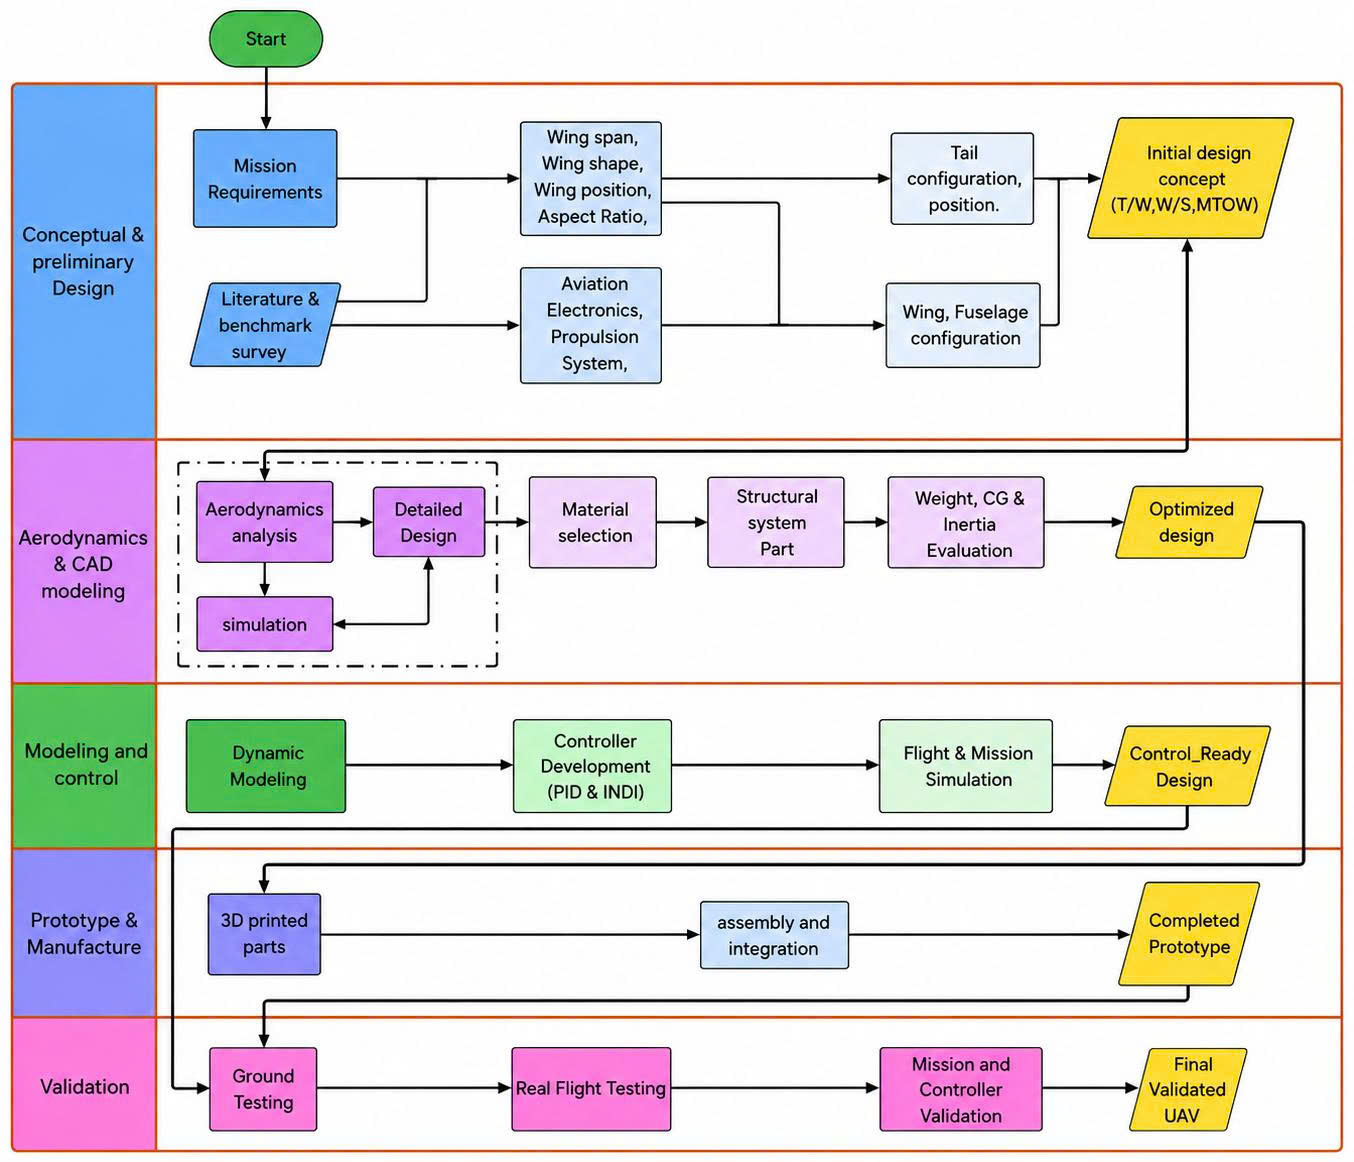
\includegraphics[width=\textwidth]{./images/Total process.jpeg}
    \caption{Overall project workflow, top-down design for prototyping and validation}
    \label{fig:total-process}
\end{figure}

\subsection{Aircraft, autopilot and simulator}
\label{sec:platform-methodology}
\label{sec:system-overview-methodology}
\label{sec:why-ardupilot}
\label{sec:sixdof-methodology}
The aircraft is a twin-boom quadplane, Fig.~\ref{fig:quadplane-concept}. A central fuselage and wing carry two tail booms. Each boom holds two lift motors and its own tail. A pusher motor on the fuselage gives thrust for cruise. The lift motors hold the aircraft in hover and give the control moments at low speed; the wing takes over as airspeed builds. The flight is therefore split into hover, transition and fixed-wing cruise (Section~\ref{sec:transition-corridor}). The assembled airframe was tested on a bench stand, Fig.~\ref{fig:stationary-bench}.

\begin{figure}[H]
    \centering
    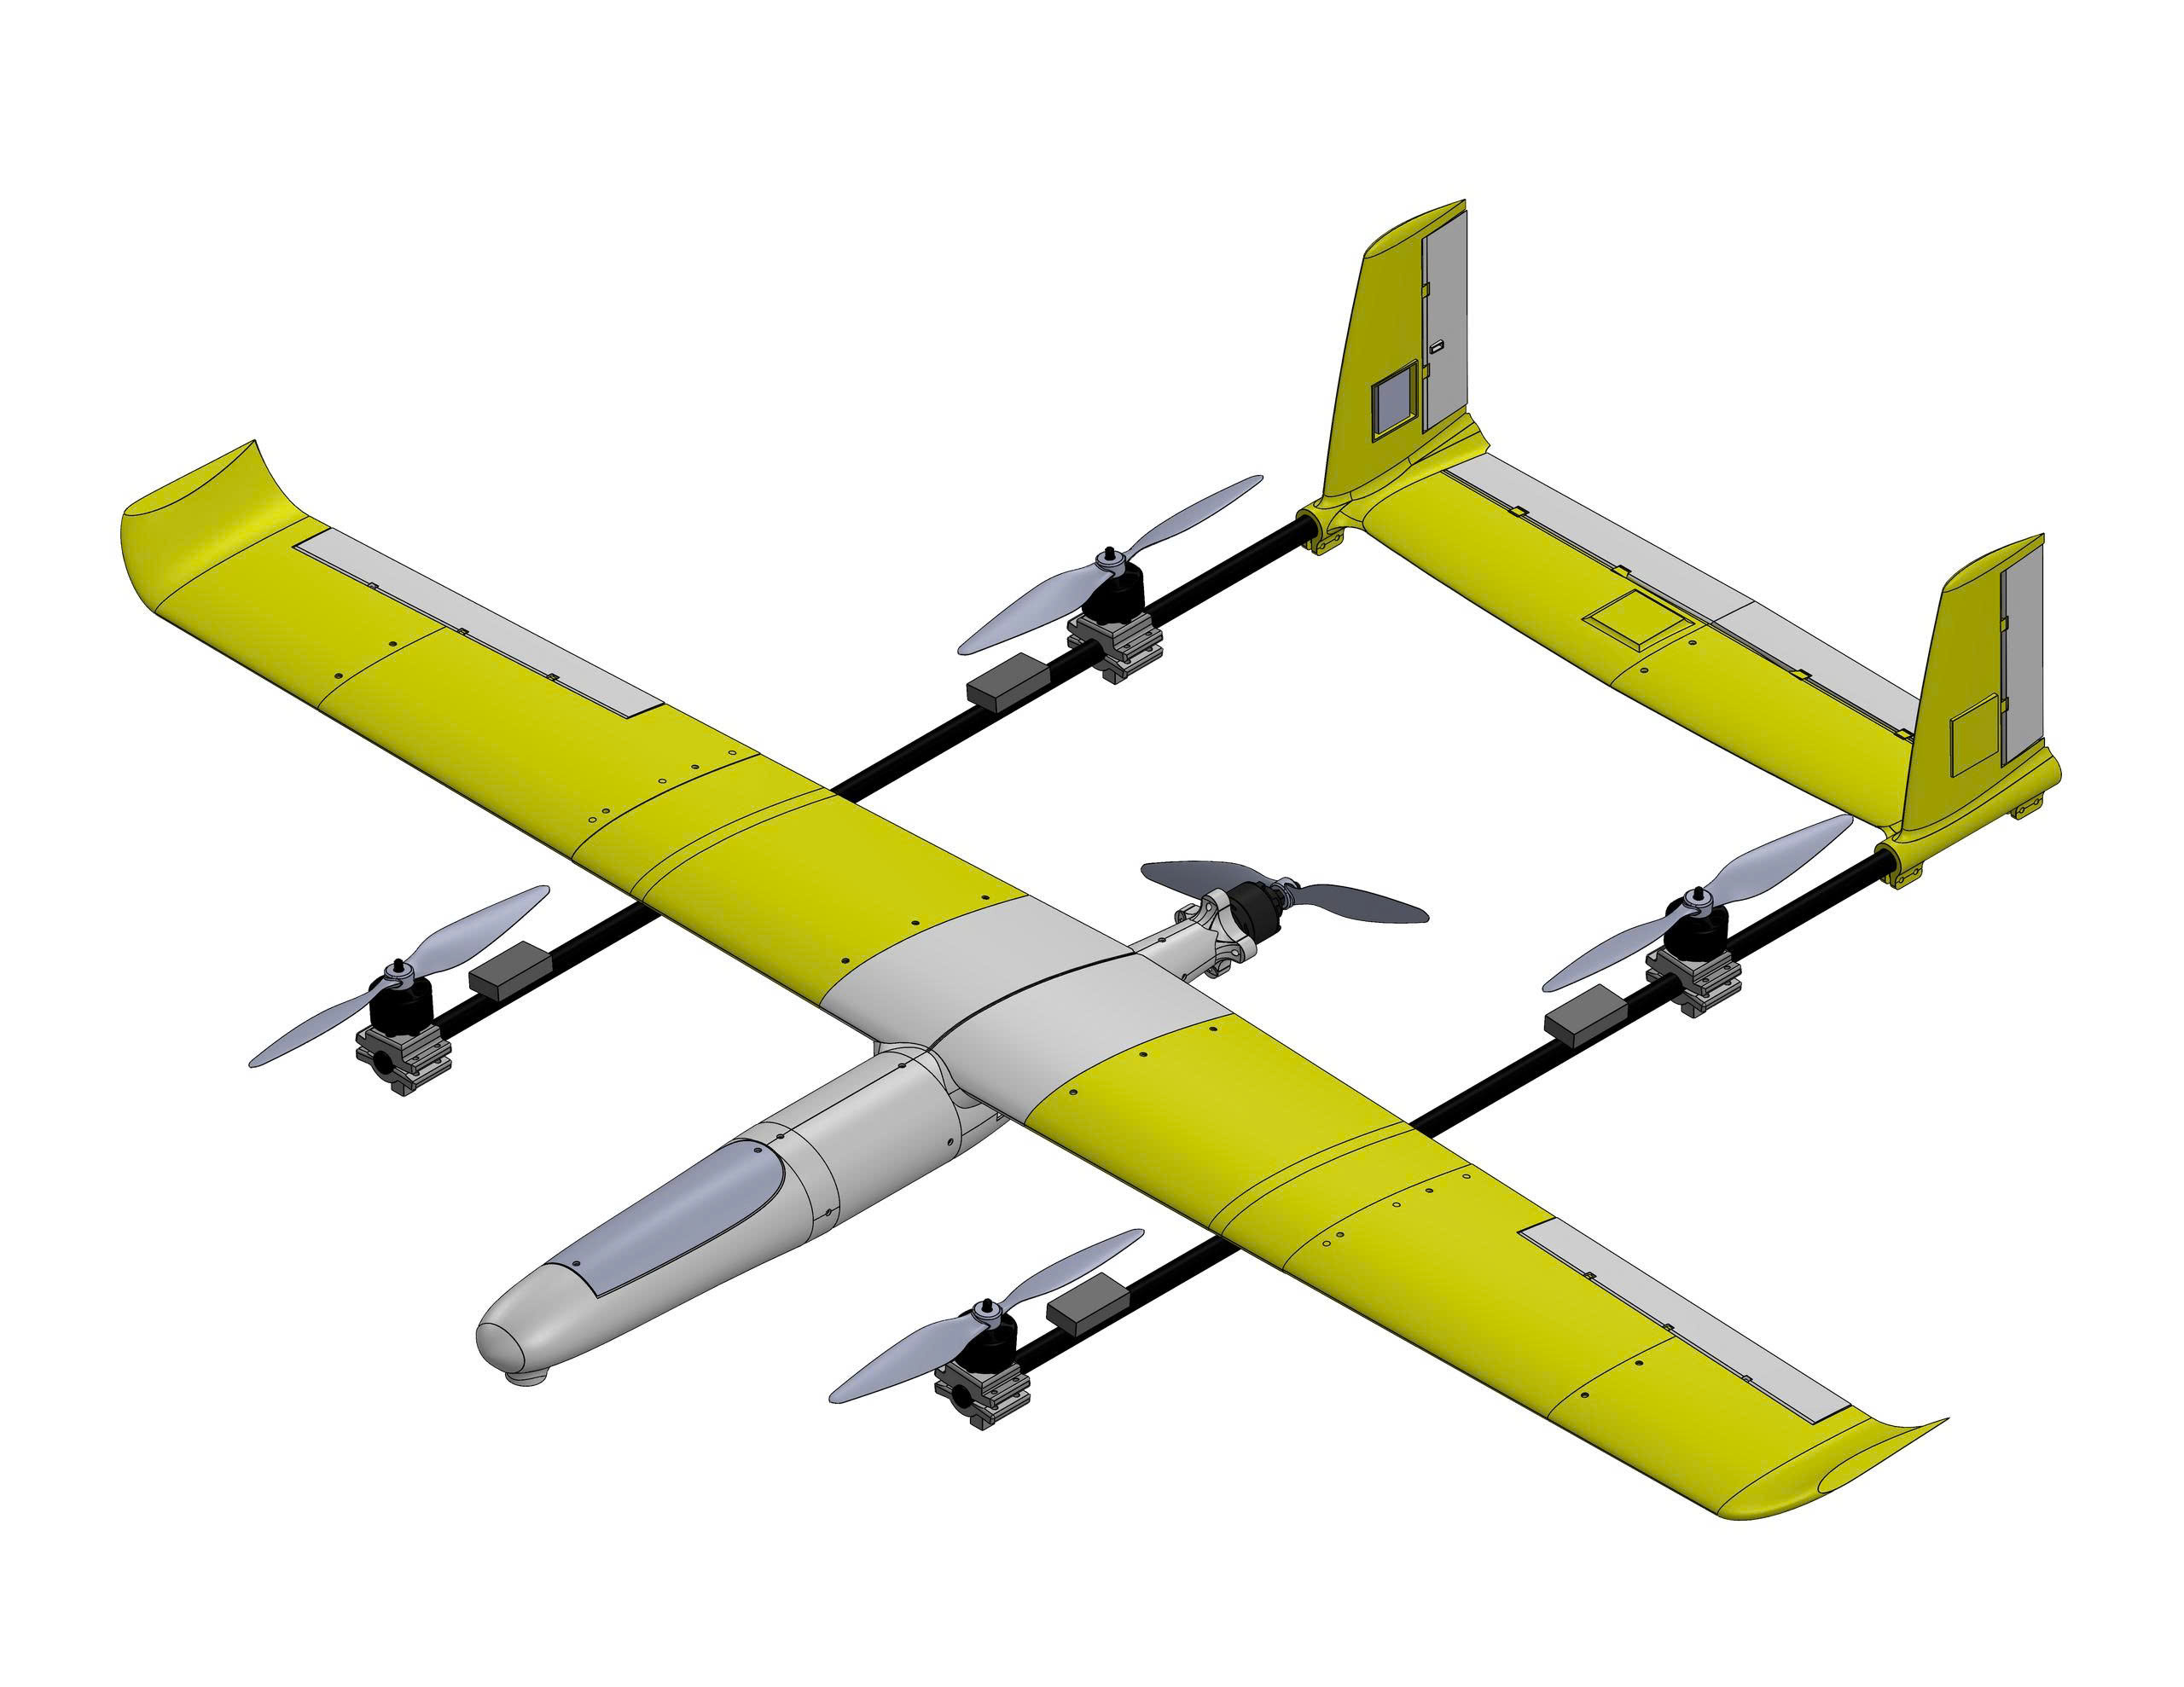
\includegraphics[width=0.75\textwidth]{./images/3D model.jpeg}
    \caption{CAD model of the twin-boom quadplane configuration: four VTOL lift motors on the booms, a forward pusher motor, and a fixed wing with an independent tail on each boom.}
    \label{fig:quadplane-concept}
\end{figure}

\begin{figure}[H]
    \centering
    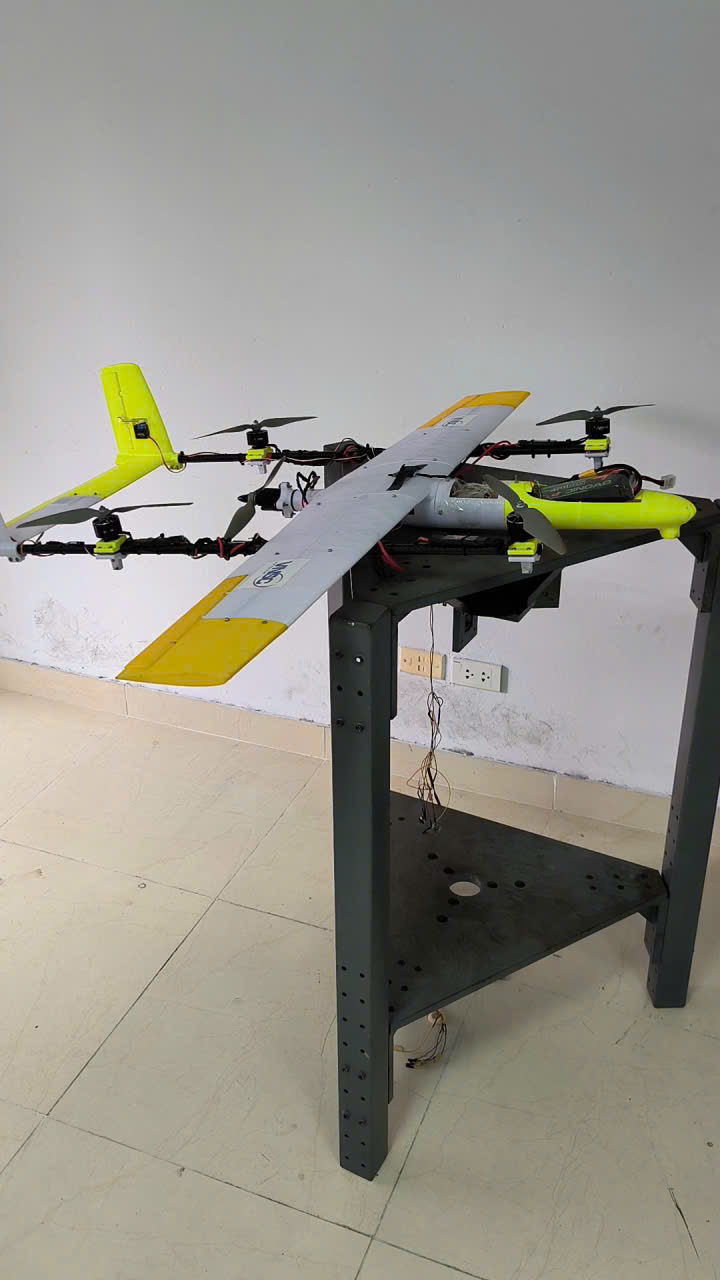
\includegraphics[width=0.85\textwidth]{./images/stationary bench.jpeg}
    \caption{Assembled airframe secured to a bench stand for ground testing.}
    \label{fig:stationary-bench}
\end{figure}

\textbf{Autopilot.} ArduPilot was chosen because it is mature, open-source flight software that already supports quadplanes. It provides, unchanged:
\begin{itemize}
    \item sensor drivers and an extended Kalman filter that estimates attitude, rates, position and velocity;
    \item the outer attitude loop, which turns a desired attitude into a desired body rate;
    \item guidance, navigation, flight modes and the transition logic between hover and wing-borne flight;
    \item the mixer, which turns roll, pitch, yaw and throttle commands into motor and servo outputs;
    \item parameter storage and flight logging;
    \item the stock PID rate loop, which stays in the code as the fallback.
\end{itemize}
Only the inner body-rate loop is replaced. Everything before it (attitude error, rate target) and after it (mixer, outputs) is stock ArduPilot. Navigation, waypoint following and altitude control are left to ArduPilot and are the same for both controllers. A boot-time switch decides whether the INDI code is loaded at all; with the switch off, the aircraft runs the stock firmware behaviour.

\textbf{Simulator.} The same ArduPilot source is compiled for a desktop computer (software-in-the-loop, SITL) and connected to Gazebo, which computes the rigid-body motion and aerodynamic forces. A bridge passes motor and servo commands one way and IMU, barometer, GPS and airspeed data the other. Real and simulated flights produce the same log format, so one analysis pipeline reads both.

\textbf{Frames.} The body frame is forward-right-down, as in Section~\ref{sec:sixdof} and in ArduPilot. Gazebo uses east-north-up world axes, so the bridge converts between the two. A sign error here would reverse the aerodynamic and propulsive terms of Eqs.~\eqref{eq:translation}--\eqref{eq:rotation}, and the controller would look unstable when the fault is in the model interface.

\subsection{Aerodynamic model: from OpenVSP to Gazebo}
\label{sec:aero-model-method}
The airframe geometry was built in OpenVSP \citep{openvspdocs}. Its vortex-lattice solver swept angle of attack and returned the lift, drag and pitching-moment coefficients of the whole aircraft, together with the reference area, span and chord. Lift and drag follow
\begin{equation}
    L=\tfrac{1}{2}\rho V^{2}SC_{L},\qquad D=\tfrac{1}{2}\rho V^{2}SC_{D}.
\end{equation}

Gazebo does not read an OpenVSP file. Its lift-drag system models each surface as one flat panel described by a handful of numbers, listed in Table~\ref{tab:liftdrag-params}. The wing, aileron sections, horizontal tail, elevator, vertical fins, rudders and winglets are each one panel, or a left and right pair. Below stall the panel lift coefficient is linear in angle of attack,
\begin{equation}
    C_L = C_{L\alpha}\,(\alpha+\alpha_0) + k_\delta\,\delta ,
    \label{eq:gazebo-lift}
\end{equation}
where $\delta$ is the deflection of the surface's control joint, if it has one. Past the stall angle the slope changes to a separate post-stall value. The OpenVSP results must be turned into these numbers by hand; the solver's own output is not used during flight. Section~\ref{sec:aero-methodology} checks how well the flown model matches the OpenVSP sweep.

\begin{table}[H]
\centering
\caption{Parameters of one Gazebo lift-drag panel, with the main-wing values of the flown model and the matching OpenVSP value where one exists. The SDF tag names are given in Appendix~\ref{sec:appendix-names}.}
\label{tab:liftdrag-params}
\begin{tabular}{llcc}
\hline
Symbol & Meaning & Main wing (flown) & OpenVSP \\
\hline
$S$ & panel area & \SI{0.183}{\meter\squared} & \SI{0.204}{\meter\squared} (whole wing) \\
$\alpha_0$ & angle added to the geometric angle of attack & \SI{0.130}{\radian} & \SI{0.049}{\radian} \\
$C_{L\alpha}$ & lift-curve slope & \SI{3.70}{\per\radian} & \SI{5.98}{\per\radian} \\
$C_{D\alpha}$ & drag-curve slope & \SI{0.064}{\per\radian} & --- \\
$C_{m\alpha}$ & pitching-moment slope & 0 & from $C_m(\alpha)$ sweep \\
$\alpha_{\mathrm{stall}}$ & stall angle & \SI{0.339}{\radian} (\ang{19.4}) & not modelled \\
$C_{L\alpha,\mathrm{stall}}$ & lift slope after stall & \SI{-3.85}{\per\radian} & not modelled \\
$C_{D\alpha,\mathrm{stall}}$ & drag slope after stall & \SI{-0.92}{\per\radian} & not modelled \\
$\mathbf{r}_{cp}$ & centre of pressure, body frame & (0.061, 0, 0.004) \si{\meter} & --- \\
$\hat{\mathbf{e}}_f,\hat{\mathbf{e}}_u$ & panel forward and upward axes & $+x$, $+z$ & --- \\
$k_\delta$ & lift coefficient per radian of deflection & --- (ailerons, elevator: $-5$) & --- \\
\hline
\end{tabular}
\end{table}

Each propeller is modelled the same way: two small lift-drag panels on a spinning link. ArduPilot commands the rotor speed, and the panels give a thrust that grows with the square of that speed.

\subsection{Rate controllers}
\label{sec:pid}
\label{sec:indi-implementation}
\textbf{PID baseline.} The stock loop compares the desired body rate with the measured rate and outputs a normalised command per axis,
\begin{equation}
    u(t)=K_Pe(t)+K_I\int_0^t e(\tau)\,d\tau+K_D\frac{de(t)}{dt},
    \label{eq:pid}
\end{equation}
where $e$ is the rate error. The mixer turns the three commands and the throttle into motor and servo outputs. The PID runs are the stock firmware with the INDI switch off.

\textbf{INDI law.} INDI needs one model number per axis, the control effectiveness $G$: the change in angular acceleration per unit change of normalised command,
\begin{equation}
    \Delta\dot\omega = G\,\Delta u .
    \label{eq:effectiveness}
\end{equation}
Each axis (roll, pitch) then runs the same incremental law every control cycle:
\begin{align}
    \nu &= K\,(\omega_{\mathrm{ref}}-\omega) && \text{desired angular acceleration} \nonumber\\
    \dot\omega_f &= H\!\left(\tfrac{d\omega}{dt}\right) && \text{measured angular acceleration} \nonumber\\
    u_{0,f} &= H\!\left(F_g\!\left(A\,(u_{\mathrm{applied}})\right)\right) && \text{effector state, delayed to match} \nonumber\\
    u &= u_{0,f} + \frac{\nu-\dot\omega_f}{G} && \text{new command}
    \label{eq:diagonal-inversion}
\end{align}
The derivative is a backward difference of the gyro rate. $H$ is a low-pass filter with two equal poles at \SI{12.7}{\hertz}. $A$ is a model of the effector: a pure delay followed by a first-order lag. $F_g$ is a copy of the gyro filter that ArduPilot applies before the rate reaches the controller.

\textbf{Why the command path is filtered.} The incremental relation of Eq.~\eqref{eq:indi-taylor-simplified} compares an acceleration with the command that caused it. The measured acceleration has passed through the effector lag, the gyro filter and $H$. The command $u_{\mathrm{applied}}$ is therefore passed through the same three stages, $A$, $F_g$ and $H$, so that both signals arrive at the subtraction with the same delay:
\begin{equation}
    u_{0,f} = H\,F_g\,A\;u_{\mathrm{applied}} .
    \label{eq:sync-fix}
\end{equation}
Filtering with $H$ alone was not enough; the loop limit-cycled until all three stages were matched (Section~\ref{sec:filtering-problem}). $u_{\mathrm{applied}}$ is what the mixer actually sent in the last cycle, recovered from the motor outputs, so saturation and mixer limits are included.

\textbf{Effectiveness.} For the lift motors, $G$ is a fixed value per axis, identified in hover (Section~\ref{sec:results-identification}). For the control surfaces the moment grows with dynamic pressure, so
\begin{equation}
    G_s(V) = G_{s,\mathrm{ref}}\left(\frac{V}{V_{\mathrm{ref}}}\right)^{2},
    \label{eq:fw-indi-scaling}
\end{equation}
with $G_{s,\mathrm{ref}}$ identified at the reference airspeed $V_{\mathrm{ref}}=\SI{15}{\meter\per\second}$. Yaw stays on the PID in both cases: its effectiveness could not be identified (Section~\ref{sec:results-yaw}).

\subsection{Which effector runs INDI, and when}
\label{sec:indi-fw-implementation}
A quadplane has two sets of effectors for roll and pitch: the lift motors and the control surfaces. ArduPilot already decides, every cycle, which rate loop drives which set. It uses its transition logic: whether the aircraft is in a hover mode, whether the forward transition has finished, and whether the lift motors are currently helping the wing (``assist''). This project does not change that decision. It only replaces the PID with INDI on the set that ArduPilot has put in charge, following the rule below.

\begin{lstlisting}[style=pseudostyle, caption={Effector ownership, evaluated every control cycle.}, label={lst:ownership}]
if hover mode, or transition not finished, or lift motors assisting:
    lift motors  -> INDI  (roll, pitch)
    surfaces     -> stock PID
else:                                   # wing-borne flight
    lift motors  -> off
    surfaces     -> INDI  (roll, pitch)
yaw              -> stock PID, always
any axis with G = 0, or motors not spun up -> stock PID
\end{lstlisting}

The rule gives one property by construction: at any instant at most one INDI loop acts on an axis. Two INDI loops acting together would each invert the same acceleration error, and the aircraft would receive twice the intended correction. The cost is that during the transition the surfaces are driven by the PID while the motors are driven by INDI, so the surface moment is an unmodelled input for the motor INDI loop. INDI measures the resulting acceleration and corrects it at the next step, which is the robustness argument of Section~\ref{sec:indi-theory}, but it is not a joint allocation. The internal names of this decision in ArduPilot are listed in Appendix~\ref{sec:appendix-transition-hooks}.

When INDI is not running on an axis, its states follow the PID output, so a later switch to INDI starts from the current command without a jump.

% The earlier text of this subsection described a joint allocation between lift
% motors and surfaces (pseudo-inverse over G_m and G_s, thrust-scaled G_m). That
% is not what the code on branch `indi` does; it was replaced by the handover
% rule above. Kept here for reference only.
% \subsubsection*{One law, allocated between effectors} ...

\subsection{Simulation set-up and flight profiles}
\label{sec:sim-to-real}
\label{sec:mission-profile}
Each case runs in its own folder with a fresh autopilot memory, so no setting carries over from the previous run. Every parameter is checked afterwards against the values the autopilot wrote into its log at boot. Each case archives the log, the world file, the parameter file, the console output and a short summary of whether the aircraft armed, transitioned, reached every waypoint and landed. Two missions are flown, Table~\ref{tab:profiles}.

\textbf{Square circuit.} Vertical take-off to \SI{35}{\meter}, a closed square of about \SI{250}{\meter} per side, and a vertical landing at the take-off point. One circuit contains every phase: hover, forward transition, wing-borne flight with four \ang{90} turns, back transition, and hover. Because the aircraft flies all four headings, one steady wind is a crosswind, headwind, opposite crosswind and tailwind in turn, all in one log.

\textbf{Zigzag.} A lawn-mower pattern to test quick turns: five parallel legs of \SI{500}{\meter}, \SI{100}{\meter} apart, flown alternately north and south (heading \ang{356} and \ang{176}) at \SI{35}{\meter} and \SI{16.1}{\meter\per\second}. Each leg runs \SI{10}{\meter} past its end before the turn. The four turnarounds are each two \ang{90} turns \SI{100}{\meter} apart, so the aircraft reverses direction in a short distance and the roll axis is loaded far more often than on the square. The plan ends with a landing at the far corner of the pattern, about \SI{765}{\meter} from the take-off point.

\begin{table}[H]
\centering
\caption{Flight profiles. Both are read directly from their mission files, so the desired path in every figure and the flown mission come from the same source.}
\label{tab:profiles}
\begin{tabular}{lcc}
\hline
 & Square circuit & Zigzag \\
\hline
Legs & 4 $\times$ \SI{250}{\meter} & 5 $\times$ \SI{500}{\meter}, \SI{100}{\meter} apart \\
Turns & 4 $\times$ \ang{90} & 4 $\times$ \ang{180} (each two \ang{90}) \\
Altitude & \SI{35}{\meter} & \SI{35}{\meter} \\
Landing & at take-off point & far end, \SI{765}{\meter} away \\
Tests & all phases, all wind headings & repeated quick turns \\
\hline
\end{tabular}
\end{table}

\textbf{Airspeed settings.} A quadplane switches its lift motors on to help the wing (``assist'') whenever it believes the airspeed is too low. In the earlier campaign a setting forced this help on for the whole flight, and the speed limits were above what the aircraft could reach. The ``fixed-wing'' part of every earlier run was therefore flown with the lift motors running, and no surface controller was ever tested on the wing alone. The speed limits were re-set from the model's stall speed (Section~\ref{sec:aero-methodology}):
\begin{itemize}
    \item stall speed \SI{12}{\meter\per\second};
    \item minimum airspeed \SI{14}{\meter\per\second};
    \item lift-motor assist only below \SI{13}{\meter\per\second}, as a low-speed safety net, and the forced-assist setting cleared;
    \item cruise \SI{17}{\meter\per\second}, which the model holds.
\end{itemize}

\subsection{Wind and disturbance injection}
\label{sec:wind-injection}
Wind is set in the Gazebo world file as one steady vector per case, with small turbulence (\SI{0.3}{\meter\per\second} in magnitude, \SI{0.02}{\radian} in direction, \SI{0.05}{\meter\per\second} vertically). Three things must hold for the wind to be real, and each failed at some point in this work:
\begin{enumerate}
    \item \emph{The aerodynamics see the wind.} Each lift-drag panel computes its own air-relative velocity from the world wind.
    \item \emph{The wind does not also push the body.} Gazebo's default wind plugin adds a drag force $F=m(\mathbf{v}_w-\mathbf{v})$, about \SI{48}{\newton} at cruise for this aircraft, which stops the transition. This force is switched off; the panels already produce the aerodynamic drag.
    \item \emph{The autopilot sees the same wind.} The bridge now sends the wind vector to ArduPilot, so its airspeed is air-relative and not ground speed.
\end{enumerate}
The crab angle in crosswind checks that all three hold (Section~\ref{sec:results-wind}).

The disturbance is a torque applied directly to the airframe in Gazebo. Its size is the rolling moment of a gust of the same speed as the wind acting on one half of the wing, $M=\tfrac12\rho u^2 S\,b/4$: \SI{1.44}{\newton\meter} for the \SI{6}{\meter\per\second} case and \SI{3.24}{\newton\meter} for \SI{9}{\meter\per\second}.

\subsection{Test configuration and scenarios}
\label{sec:test-scenarios}
Each profile is flown by both controllers in three conditions, Table~\ref{tab:test-matrix}. Conditions 2 and 3 add moment pulses on top of the wind, Table~\ref{tab:disturbance-points}. Condition 1 has neither and is the baseline.

\begin{table}[H]
\centering
\caption{Test matrix. Every case uses the same aircraft model and mission; PID and INDI differ only in the INDI parameter block. Wind speed is also given as a fraction of the \SI{17}{\meter\per\second} cruise airspeed.}
\label{tab:test-matrix}
\begin{tabular}{lcccc}
\hline
Condition & Wind [\si{\meter\per\second}] & Wind [\si{\kilo\meter\per\hour}] & Fraction of cruise & Moment pulse \\
\hline
1 calm      & 0 & 0    & ---               & none \\
2 moderate  & 6 & 21.6 & \SI{35}{\percent} & \SI{1.44}{\newton\meter} \\
3 strong    & 9 & 32.4 & \SI{53}{\percent} & \SI{3.24}{\newton\meter} \\
\hline
\end{tabular}
\end{table}

\begin{table}[H]
\centering
\caption{Moment-pulse schedule, conditions 2 and 3. Each window starts a fixed time after an autopilot event, measured on the vehicle clock, so PID and INDI receive the pulses at the same point of the mission. Each window is a roll pulse, \SI{4}{\second} rest, then a pitch pulse: eight pulses per run.}
\label{tab:disturbance-points}
\begin{tabular}{lll}
\hline
Window & Starts & Pulses \\
\hline
Take-off hover & \SI{4}{\second} after take-off begins & roll, pitch \\
Transition & \SI{3}{\second} after transition starts & roll, pitch \\
Fixed-wing & \SI{3}{\second} after the fourth waypoint & roll, pitch \\
Landing hover & \SI{5}{\second} after landing descent starts & roll, pitch \\
\hline
\multicolumn{3}{l}{Pulse: \SI{1}{\second}, body axis, magnitude from Table~\ref{tab:test-matrix}.} \\
\hline
\end{tabular}
\end{table}
% User asked (2026-09-26) for 1.44 N.m pulses at every corner and leg midpoint.
% The flown campaign (sim/fly_plan_mission.py, class Disturbance) uses the
% event windows above and 3.24 N.m at 9 m/s. Change the text if the campaign
% is re-flown with the corner/midpoint schedule.

The altitude controller is ArduPilot's in both cases; the INDI build adds nothing to the vertical loop. Each log is split into hover, forward transition, wing-borne flight, back transition and landing from the logged transition state, airspeed and lift-motor output, with the same rule for PID and INDI.

\subsection{Metrics and analysis procedure}
\label{sec:metrics}
The pipeline reads each log, keeps the recorded units, and splits the mission into phases. ArduPilot logs body rates in \si{\degree\per\second}; an earlier analysis converted them from radians a second time and overstated every rate error by $180/\pi$. Each phase interval is filtered and transformed separately, so the jump between two windows cannot create false high-frequency energy. For $N$ logged error samples $e_k$, the tracking error is
\begin{equation}
    \mathrm{RMSE}=\sqrt{\frac{1}{N}\sum_{k=1}^{N} e_k^2}.
    \label{eq:rmse}
\end{equation}
The stability measure is the RMS angular acceleration from the gyro over \SIrange{6}{60}{\hertz}. It uses the gyro, which both controllers share, rather than a signal that exists only inside INDI. Pseudo-control tracking is tested below \SI{5}{\hertz} on each phase interval: correlation tests direction and $\mathrm{RMS}(\dot\omega_f)/\mathrm{RMS}(\nu)$ tests amplitude. Other metrics are attitude and rate RMSE, cross-track error, the share of commands above 0.95 of full scale, crab angle, and the fraction of time each axis runs INDI.

The comparison is paired: same mission, same wind, same pulses, only the controller changes. Once the two controllers respond differently their paths also differ, so later parts of a run are no longer a strictly controlled comparison. Differences smaller than the spread across repeated seeds are not claimed as results.

\section{Results and Discussion}
\label{sec:results}

\subsection{What the real flight log can and cannot establish}
\label{sec:results-baseline}
The one physical-flight record available is a \SI{157.1}{\second} stock-PID log. Mode segmentation gives hover mode from \SIrange{7.8}{112.1}{\second}, stabilised fixed-wing mode from \SIrange{112.1}{120.5}{\second}, and hover mode again to the end. Thus only \SI{8.4}{\second}, or \SI{5}{\percent}, is fixed-wing operation. Ground speed in that fixed-wing interval averaged \SI{3.7}{\meter\per\second} and reached \SI{5.9}{\meter\per\second}; the logged airspeed reached only \SI{6.0}{\meter\per\second}, well below the \SI{16}{\meter\per\second} minimum-airspeed setting. The log contains no airspeed-sensor messages. The physical aircraft was therefore not demonstrably wing-borne, and the recorded fixed-wing interval cannot validate the transition corridor or the wing model.

\begin{figure}[H]
    \centering
    \includegraphics[width=0.98\textwidth]{../../data/plots/thesis/F1_real_overview.pdf}
    \caption{Purpose: establish the operating envelope of the only physical-flight dataset before using it for validation. The flight is predominantly in hover mode; the short fixed-wing interval remains below \SI{6}{\meter\per\second}. This plot is the evidence for excluding real transition and cruise validation from the present study.}
    \label{fig:real-flight-overview}
\end{figure}

The log does provide three useful hardware facts. First, the learned hover throttle and the stored hover-throttle setting both equal 0.408, providing a configuration and hover-estimator consistency check. Second, it records the real scheduler rate (\SI{300}{\hertz}), the \SI{42}{\hertz} gyro filter, and the vibration spectrum quantified in Table~\ref{tab:vibration}. Third, it shows the actuator and sensor logging needed for a future matched PID experiment. These are constraints on the simulation and controller design; they are not proof that Gazebo reproduces the real rigid-body or aerodynamic response.

Conversely, this dataset cannot support aerodynamic trim validation, transition tracking validation, control-effectiveness identification, gust-rejection performance, or a hardware PID-versus-INDI comparison. Fixed-wing trim requires measured airspeed and a sustained segment long enough to average the phugoid; both are absent. The hand-flown rate content also lacks the independent, band-limited excitation needed to identify the inner-loop plant. The defensible result is consequently a constrained sim-to-real assessment: the simulation under-represents the differentiated-gyro noise substantially, while dynamic fidelity over the transition and cruise envelope remains unvalidated.

Figure~\ref{fig:descriptive-pid-rates} places representative real and simulated PID hover-rate traces beside one another to show why time-domain appearance alone is not a validation metric. The real window has roll and pitch RMS rate errors of \SI{4.67}{\degree\per\second} and \SI{5.52}{\degree\per\second}; the autonomous calm-SITL window has \SI{0.30}{\degree\per\second} and \SI{2.19}{\degree\per\second}. The windows have different commands, noise, and pilot/autopilot excitation, so the smaller simulated values cannot be attributed to a more accurate model or better controller. Their purpose is descriptive: they show the data available and motivate the matched experiment still required.

\begin{figure}[H]
    \centering
    \includegraphics[width=0.98\textwidth]{../../data/plots/thesis/F2_rate_tracking.pdf}
    \caption{Purpose: show representative PID rate tracking in the real and simulated hover records. The panels are deliberately labelled as an unmatched descriptive comparison; their RMS values must not be read as an A/B controller result.}
    \label{fig:descriptive-pid-rates}
\end{figure}

\subsection{Baseline simulated mission path}
\label{sec:results-pid-path}
% REVIEW[P0] R-12: this subsection describes the out-and-back mission. The campaign
% now flies the closed 250 m square circuit of Section~\ref{sec:mission-profile};
% re-generate from logs/{pid,indi}_{calm,cross6,cross9}.BIN.
The calm and wind-enabled PID mission runs provide the geometric baseline for the rest of the study. Fig.~\ref{fig:pid-flight-path} shows the commanded rectangular path against the simulated vehicle track under a \SI{5}{\meter\per\second} wind and a \SI{19}{\meter\per\second} cruise setting. The plot is useful because it shows that the simulator and mission scripts can complete the same end-to-end profile used later for the INDI comparison, including the transition into and out of forward flight. It does not, by itself, establish that the plant model is correct or that the real vehicle would follow the same path.

\begin{figure}[H]
    \centering
    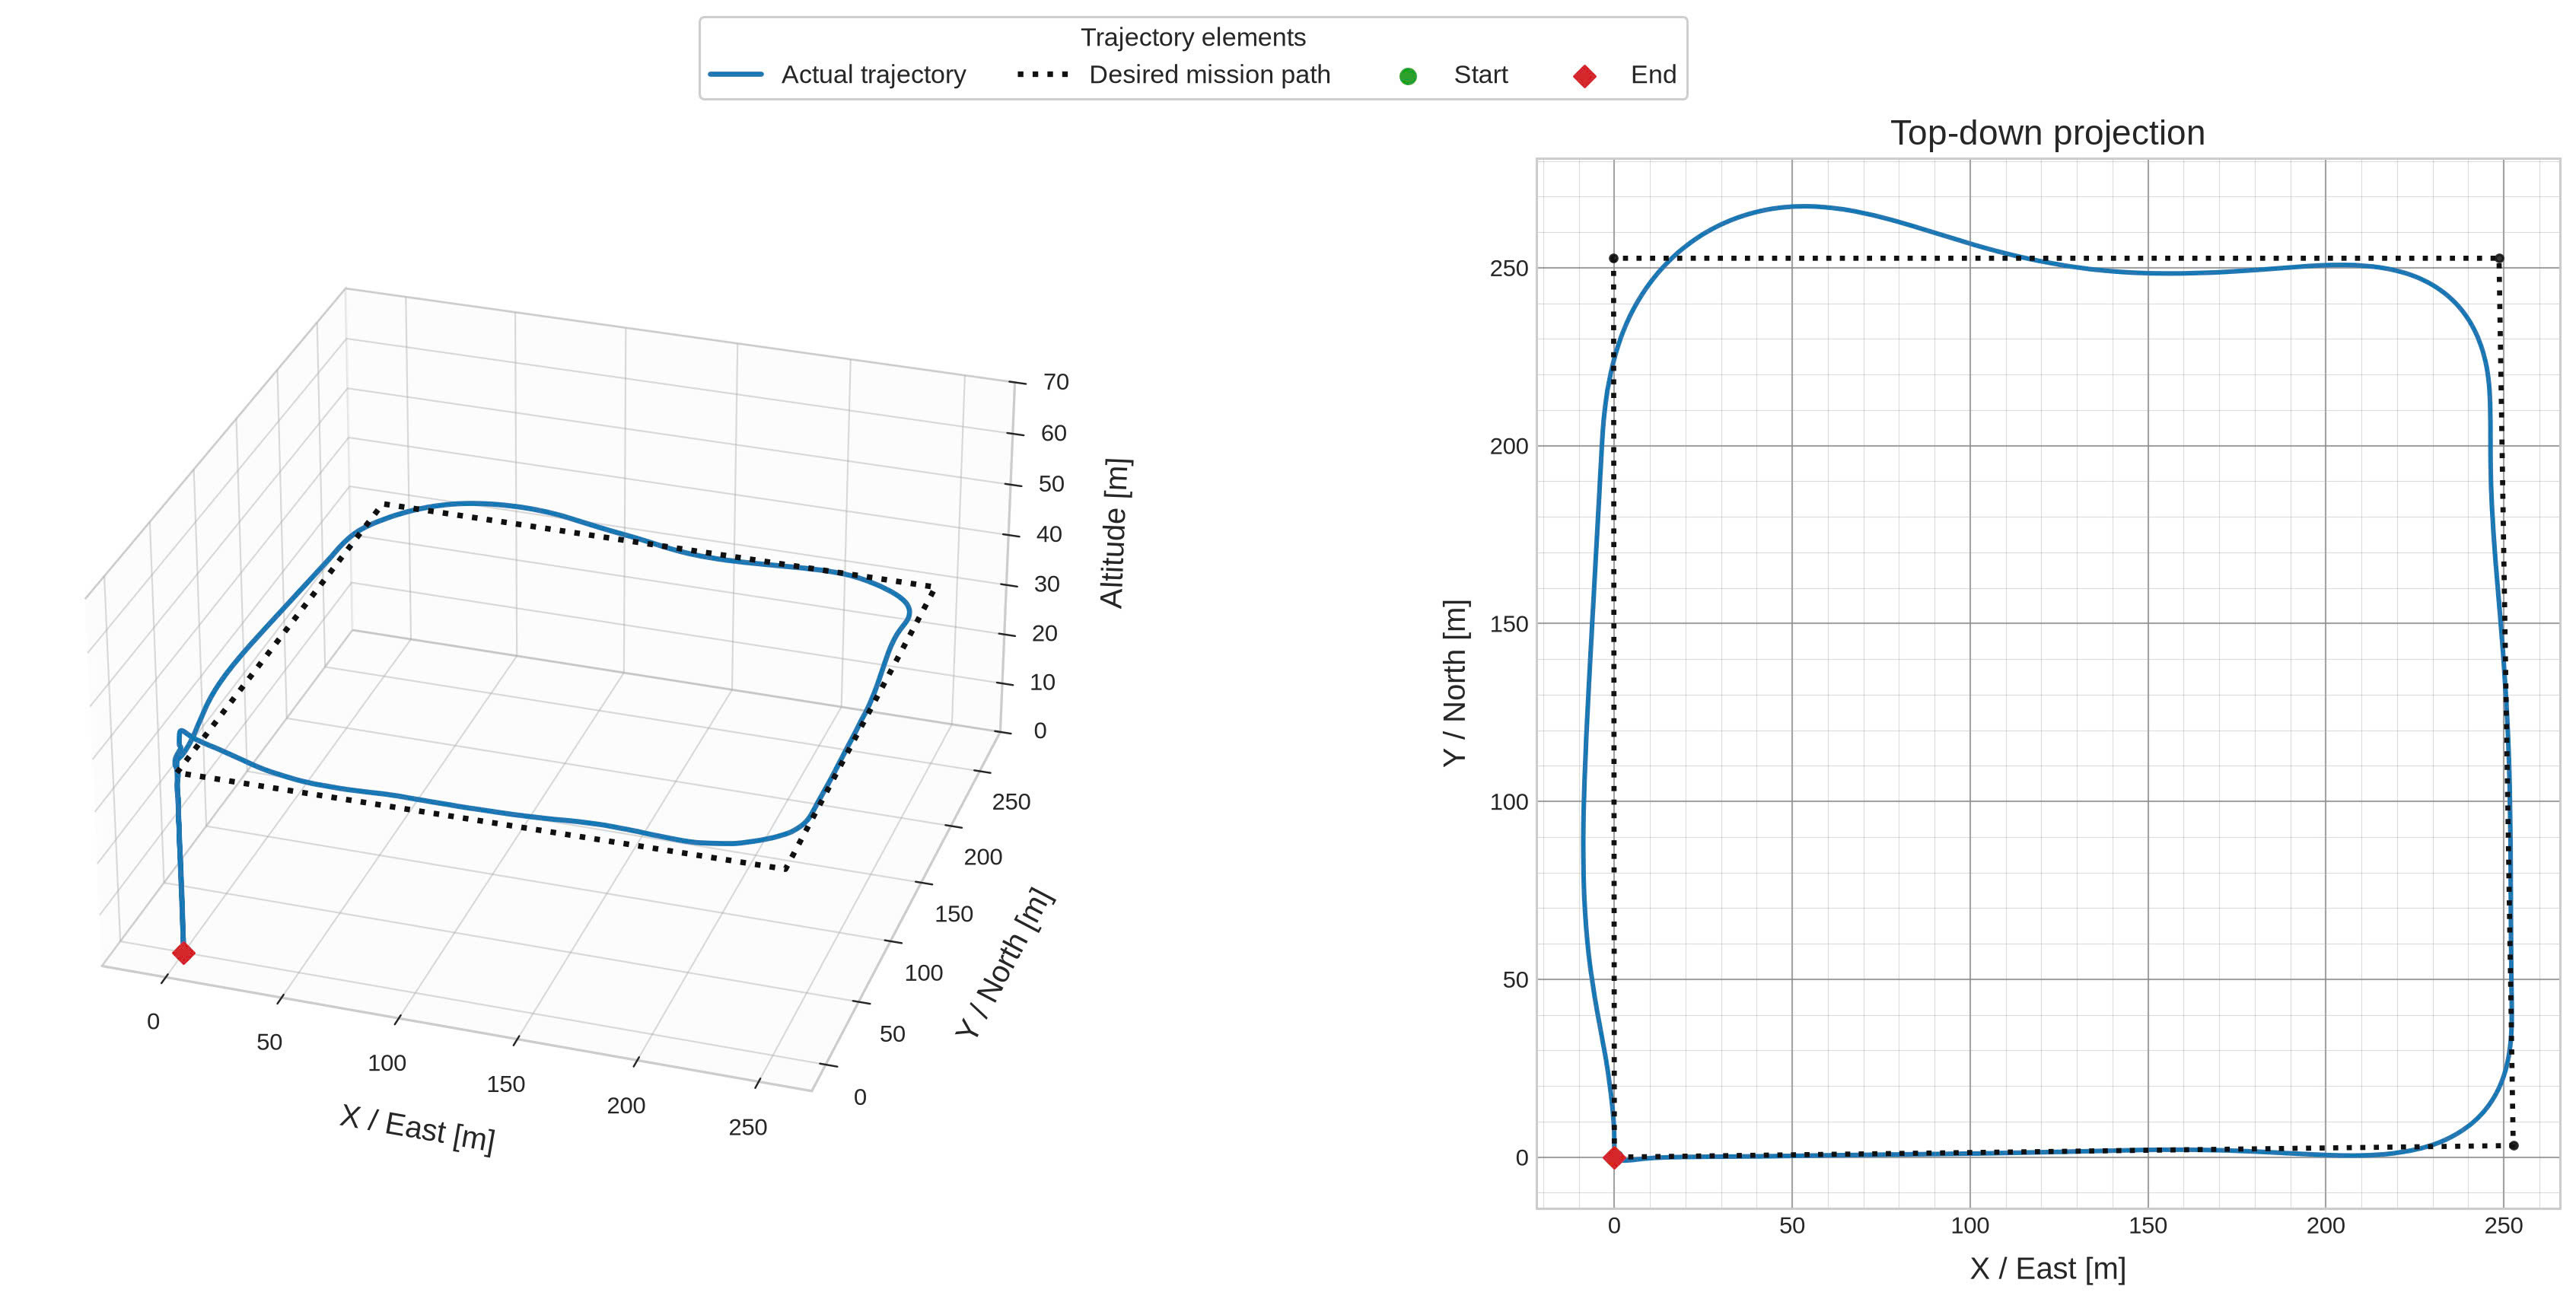
\includegraphics[width=0.98\textwidth]{./images/PID flight path - 5ms wind, 19ms cruise speed.jpeg}
    \caption{Simulated PID trajectory tracking versus the desired mission path, 3D view (left) and top-down projection (right), under a \SI{5}{\meter\per\second} wind at \SI{19}{\meter\per\second} cruise airspeed.}
    \label{fig:pid-flight-path}
\end{figure}

\subsection{Aerodynamic model}
\label{sec:aero-methodology}
\label{sec:yaw-authority-methodology}
Figure~\ref{fig:aero-performance} shows the OpenVSP sweep of the full airframe and Fig.~\ref{fig:wing-vector-field} the pressure field near the fuselage/wing junction. These are not flight results. They are the reference against which the Gazebo model is checked.

\begin{figure}[H]
    \centering
    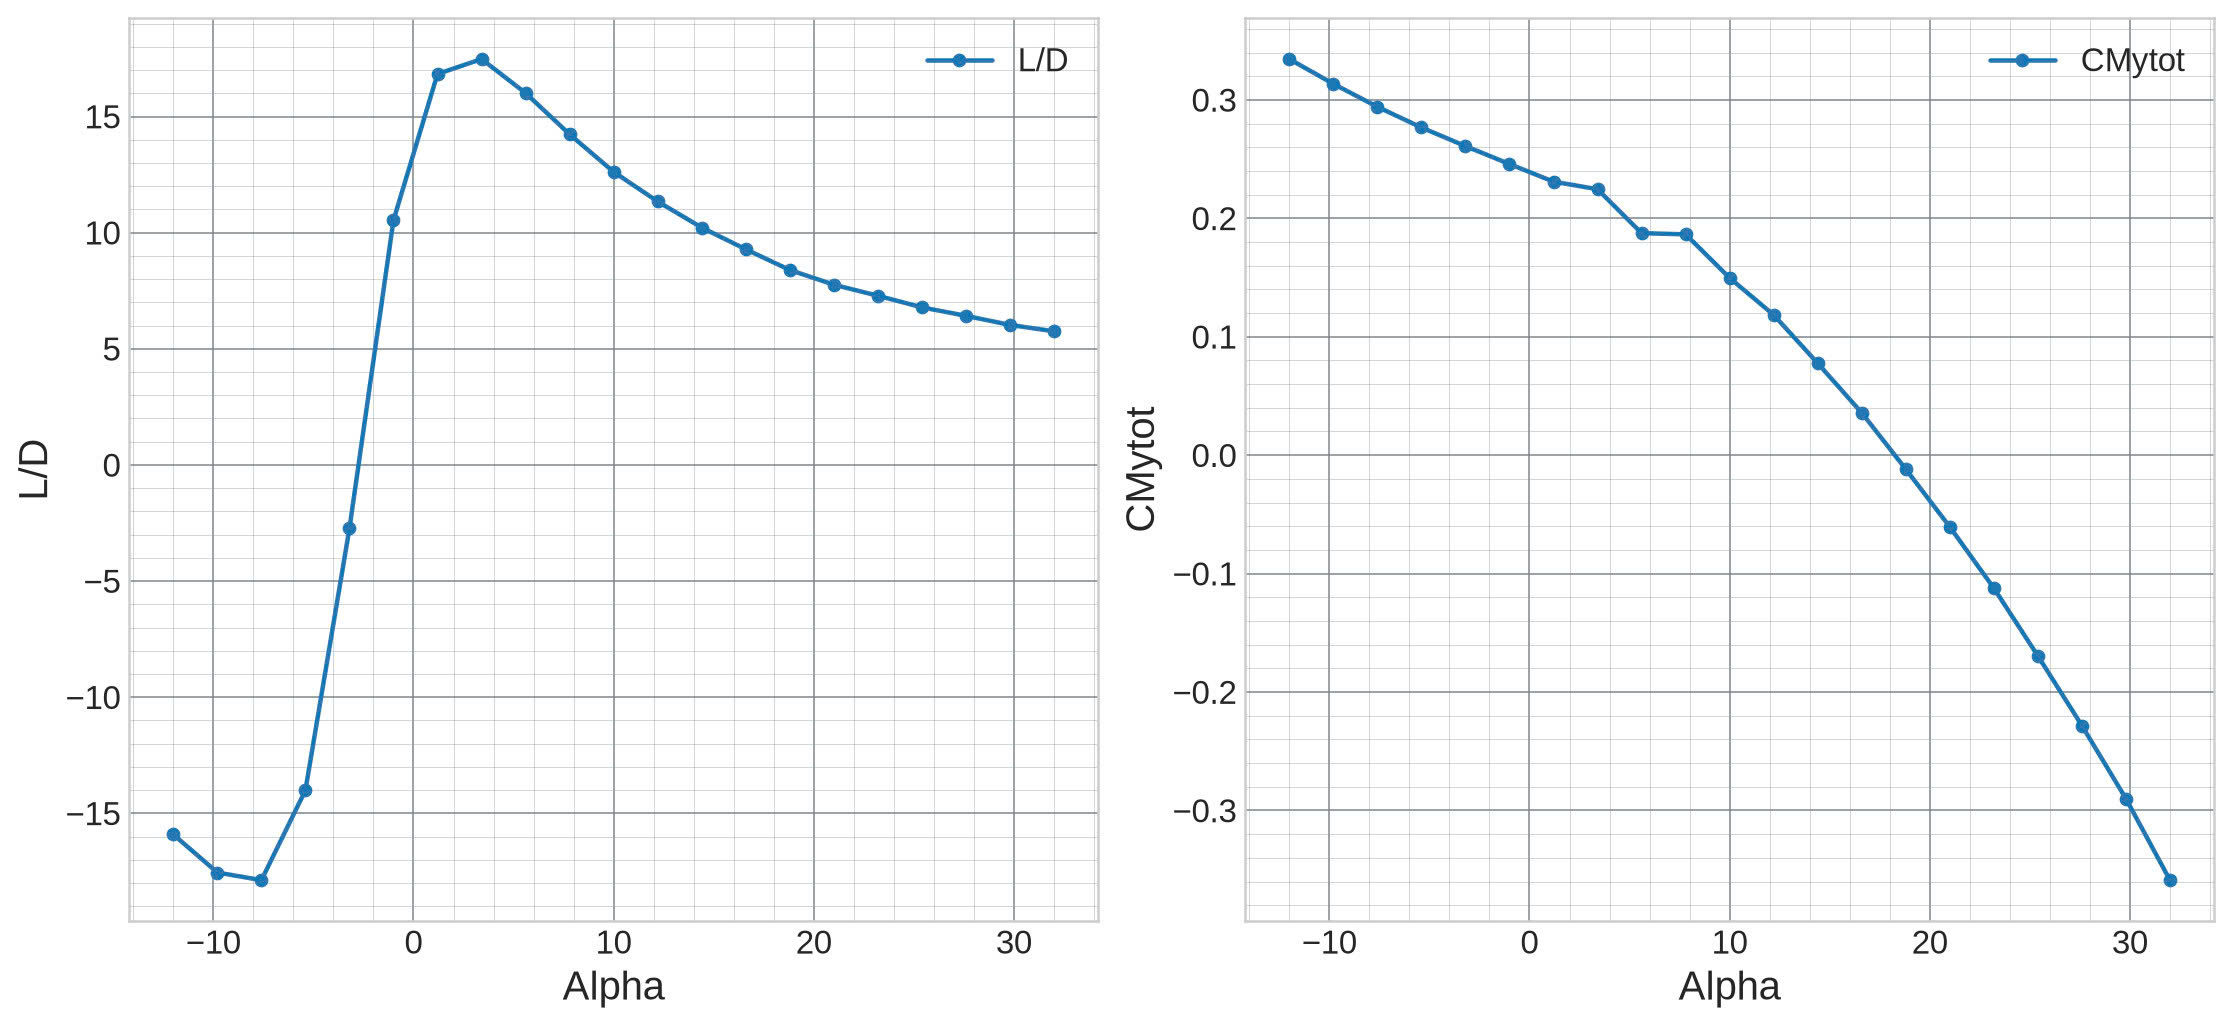
\includegraphics[width=\textwidth]{./images/aerodynamic performance.jpeg}
    \caption{OpenVSP-derived aerodynamic performance of the full airframe: lift-to-drag ratio and total pitching-moment coefficient versus angle of attack $\alpha$ (deg).}
    \label{fig:aero-performance}
\end{figure}

\begin{figure}[H]
    \centering
    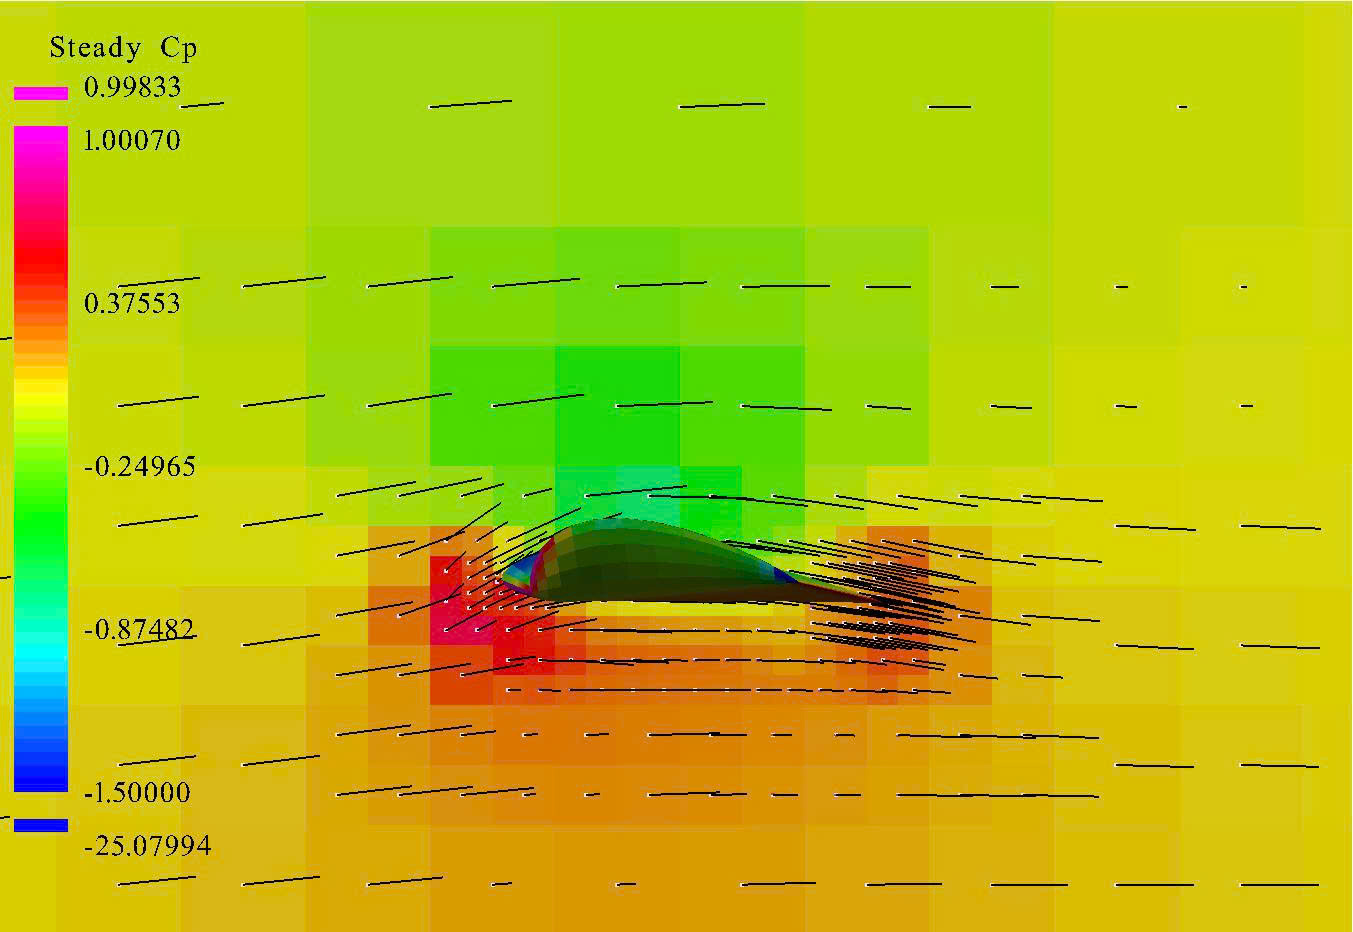
\includegraphics[width=0.7\textwidth]{./images/wing lift vector field.jpeg}
    \caption{OpenVSP surface pressure coefficient and local flow-velocity vectors near the fuselage/wing junction, used to sanity-check the centre-of-pressure location.}
    \label{fig:wing-vector-field}
\end{figure}

\textbf{Model check.} Every lift-drag panel of the flown model was ranked by the maximum lift it can make, $S\,C_{L,\max}$ with $C_{L,\max}=C_{L\alpha}\,\alpha_{\mathrm{stall}}$ (Table~\ref{tab:surface-ranking}). The script is listed in Appendix~\ref{sec:appendix-names}.

\begin{table}[H]
\centering
\caption{Lifting surfaces of the flown Gazebo model, ranked by maximum lift. Share is of the wing and horizontal-tail total, \SI{0.428}{\meter\squared}. Left and right panels are combined.}
\label{tab:surface-ranking}
\begin{tabular}{lcccccc}
\hline
Surface & $S$ [\si{\meter\squared}] & $C_{L\alpha}$ [\si{\per\radian}] & $\alpha_{\mathrm{stall}}$ & $C_{L,\max}$ & $S\,C_{L,\max}$ [\si{\meter\squared}] & Share \\
\hline
Main wing (centre panel) & 0.1832 & 3.70 & \ang{19.4} & 1.25 & 0.230 & \SI{54}{\percent} \\
Aileron sections (2)     & 0.0177 & 6.80 & \ang{36.6} & \textbf{4.35} & 0.077 & \SI{18}{\percent} \\
Elevator                 & 0.0155 & 6.80 & \ang{36.6} & \textbf{4.35} & 0.067 & \SI{16}{\percent} \\
Horizontal tail          & 0.0425 & 3.70 & \ang{19.4} & 1.25 & 0.053 & \SI{12}{\percent} \\
\hline
\end{tabular}
\end{table}

Four problems follow from the table and the model file.
\begin{enumerate}
    \item \textbf{The wing coefficients are not from OpenVSP.} The main-wing and aileron values ($\alpha_0$, $C_{L\alpha}$, $C_{D\alpha}$, $\alpha_{\mathrm{stall}}$) are identical, to every digit, to ArduPilot's example Zephyr flying-wing model. Only the areas and centres of pressure were changed, and the areas do match OpenVSP (\SI{0.201}{} against \SI{0.204}{\meter\squared}). OpenVSP gives a lift slope of \SI{5.98}{\per\radian} and a zero-lift offset of \SI{0.049}{\radian}; the model uses 3.70 and 0.130 (Table~\ref{tab:liftdrag-params}).
    \item \textbf{The aileron and elevator panels are unrealistic.} A lift coefficient of 4.35 at a stall angle of \ang{36.6} is far beyond any plain airfoil (about 1.2--1.6 at \ang{12}--\ang{16}). The elevator, a \SI{0.015}{\meter\squared} strip, can lift more than the whole horizontal tail in front of it, and the two aileron sections add \SI{33}{\percent} to the maximum lift of the wing.
    \item \textbf{No panel carries a pitching moment} ($C_{m\alpha}=0$ everywhere). The OpenVSP pitching-moment curve is not in the model; pitch stability comes only from where the panels sit.
    \item \textbf{The weight used earlier was wrong.} The earlier stall estimate used \SI{27.5}{\newton}, which is the fuselage link alone. The model's twelve links total \SI{3.184}{\kilo\gram}, a weight of \SI{31.2}{\newton}.
\end{enumerate}

With the correct weight, the 1-g stall speed $V_s=\sqrt{2W/(\rho\,\sum S C_{L,\max})}$ is \SI{15.0}{\meter\per\second} for the centre wing panel alone, \SI{13.0}{\meter\per\second} with the aileron sections, and \SI{11.0}{\meter\per\second} with every horizontal panel. In the calm INDI run the aircraft held \ang{46.9} of bank at \SI{16.75}{\meter\per\second}, which is equivalent to \SI{13.8}{\meter\per\second} in level flight, without stalling. That is below the centre-wing bound. The model can fly there only because of the extra lift of the aileron sections, whose $C_{L,\max}$ is not physical. The \SI{14}{\meter\per\second} minimum airspeed of Section~\ref{sec:mission-profile} is therefore safe in this model but would not be on an aircraft whose outer wing stalls like a real airfoil.

Two further findings concern the control surfaces. The servo scaling for the rudders gives a travel of only about \ang{0.06}, so the rudders do not move in any run; yaw in wing-borne flight comes from the fins' passive weathercock stability alone. The ailerons and elevator travel $\pm\ang{25}$.

\textbf{Propellers.} In the model each propeller is two lift-drag panels on a spinning link, so thrust grows with the square of rotor speed, $T_i=k_{T_i}\Omega_i^2$ and $Q_i=k_{Q_i}\Omega_i^2$. The constants are set by the blade panels, not by the bench measurements of Fig.~\ref{fig:stationary-bench}. Yaw moment comes from the difference in rotor drag torque, which is governed by $k_{Q_i}$ and is the least certain part of the propulsion model; this is one reason yaw stays on the PID (Section~\ref{sec:results-yaw}).
\begin{equation}
    T_i=k_{T_i}\Omega_i^2,\qquad Q_i=k_{Q_i}\Omega_i^2
    \label{eq:propeller}
\end{equation}

These problems do not affect the PID/INDI comparison directly, because both controllers fly the same model. They do limit how far any simulated result transfers to the real aircraft (Section~\ref{sec:limitations}).

\subsection{Identifying the aircraft that is being controlled}
\label{sec:results-identification}
INDI needs one number per axis, the control effectiveness $G$, and it is the only model knowledge the law uses. Leaving it as a placeholder makes every downstream result arbitrary, so it was measured.

The mission flights cannot measure it, for the same reason the real flight cannot: an aircraft flying waypoints holds attitude, so the rate loop is excited only by what the navigation loop asks for. Fitting over that band returned $G = \SI{45.7}{\radian\per\second\squared}$ on roll and nothing usable on pitch. A dedicated manoeuvre was therefore flown: a logarithmic stick sweep from \SIrange{0.2}{6}{\hertz} over \SI{40}{\second} per axis, in hover mode, with the rate loop on the \emph{PID}. Identifying against INDI would measure a loop that already contains the number being sought.

Fitting $\alpha(s)/u(s) = G/(1+s\tau)$ to the resulting frequency response gives Table~\ref{tab:identification}.

\begin{table}[H]
\centering
\caption{Control effectiveness and effector lag, identified in hover from a swept-stick manoeuvre with the rate loop on the PID.}
\label{tab:identification}
\begin{tabular}{lcccc}
\hline
Axis & $G$ [\si{\radian\per\second\squared}] & $\tau$ [\si{\milli\second}] & Coherence & Bins \\
\hline
Roll  & 61.7 & 23.0 & 0.91 & 38 \\
Pitch & 55.4 & 23.7 & 0.89 & 37 \\
\hline
\end{tabular}
\end{table}

Two independent checks support these numbers. The two axes agree on $\tau$ to within \SI{1}{\milli\second}, which is what four shared motors should give. The pitch-to-roll effectiveness ratio is 0.90, against 0.79 predicted from the model's own geometry and inertia, $\left(x_\mathrm{arm}/I_{yy}\right)/\left(y_\mathrm{arm}/I_{xx}\right)$.

The identified $\tau$ also disposes of an earlier misreading. A fit over the mission band alone had returned \SI{88}{\milli\second}; with excitation to \SI{6}{\hertz} the same aircraft returns \SI{23}{\milli\second}. A first-order model fitted to a band containing almost no high-frequency information will return whatever time constant makes the low-frequency magnitude work, and that value should not be used.

Figure~\ref{fig:effectiveness-handover} gives the identification result and its operational consequence in one plot. The upper-left panel shows the coherent command-to-angular-acceleration data and the fitted roll model, $G_\phi=\SI{61.7}{\radian\per\second\squared}$ per unit normalised command with $\tau=\SI{23.0}{\milli\second}$. The lower panel shows the scheduled motor and surface effectiveness in the calm INDI mission. Surface effectiveness rises with dynamic pressure while motor effectiveness falls as the lift motors unload. The purpose is to show how authority moves from the lift motors to the surfaces through the transition.

\begin{figure}[H]
    \centering
    \includegraphics[width=0.98\textwidth]{../../data/plots/thesis/F4_effectiveness_handover.pdf}
    \caption{Purpose: show where the simulated-aircraft inversion gain comes from and how authority is handed from lift motors to aerodynamic surfaces. The fit is from the dedicated PID sweep; the time history is from the calm INDI mission. These values are not hardware identification results.}
    \label{fig:effectiveness-handover}
\end{figure}

\subsection{The dominant sim-to-real risk: vibration in the angular-acceleration estimate}
\label{sec:vibration-risk}
INDI does not measure angular acceleration. It differentiates the gyro. Differentiation multiplies a noise component at frequency $f$ by $2\pi f$, so gyro noise far above the control bandwidth still arrives at the inversion as angular acceleration. The quantity that matters is therefore not the gyro amplitude but the angular-acceleration noise inside the band the estimator passes.

This was measured on the real aircraft from the batch-sampled gyro log, recorded at \SI{1916}{\hertz} through \SI{94}{\second} of hover. The gyro power spectrum was multiplied by $(2\pi f)^2$ and integrated over \SIrange{25}{90}{\hertz}: the lower edge sits above the rate-loop bandwidth so that rigid-body motion is excluded, and the upper edge is below the \SI{150}{\hertz} Nyquist frequency of the \SI{300}{\hertz} control loop. The same treatment was applied to the simulated aircraft in hover.

\begin{table}[H]
\centering
\caption{Angular-acceleration noise in the estimator band, \SIrange{25}{90}{\hertz}, hover. The real-aircraft column applies the \SI{42}{\hertz} gyro low-pass filter recorded in the physical log; the calm-PID SITL result uses its logged \SI{20}{\hertz} filter.}
\label{tab:vibration}
\begin{tabular}{lcccc}
\hline
Axis & Real, raw & Real, filtered & Simulated & Ratio \\
 & [\si{\radian\per\second\squared}] & [\si{\radian\per\second\squared}] & [\si{\radian\per\second\squared}] & \\
\hline
Roll  & 15.1 & \textbf{7.1} & 0.15 & \textbf{46.6} \\
Pitch &  2.6 & 1.3 & 0.21 & 6.2 \\
Yaw   &  2.0 & 1.1 & 0.09 & 11.7 \\
\hline
\end{tabular}
\end{table}

The roll axis is dominated by a spectral line near \SI{83}{\hertz}; pitch near \SI{71}{\hertz} and yaw near \SI{53}{\hertz}. Accelerometer vibration is unremarkable on the same flight (logged vibration levels of 1.25, 1.12 and \SI{1.58}{\meter\per\second\squared} with no clipping), which is why this had not been noticed: the standard vibration check looks at the accelerometers, and the problem is on the gyro, in a band that check does not examine.

The direct comparison is deliberately limited to the estimator input; it is not an end-to-end airframe-fidelity score. Even after the physical aircraft's wider gyro filter is applied, the real roll-axis acceleration noise is \SI{7.13}{\radian\per\second\squared} RMS, compared with \SI{0.153}{\radian\per\second\squared} RMS in calm PID SITL: a factor of 46.6. Figure~\ref{fig:current-vibration} shows the spectra from which those integrals are computed. This mismatch is large enough that a rate-loop cutoff or increment limit accepted in this simulator cannot be transferred to the aircraft without hardware vibration measurements.

\begin{figure}[H]
    \centering
    \includegraphics[width=0.98\textwidth]{../../data/plots/thesis/F3_vibration.pdf}
    \caption{Purpose: quantify the differentiated-gyro environment that enters the INDI inversion. The shaded \SIrange{25}{90}{\hertz} band is integrated in Table~\ref{tab:vibration}. The result validates only the sensor-noise mismatch; it does not validate rigid-body or aerodynamic dynamics.}
    \label{fig:current-vibration}
\end{figure}

Three consequences follow. First, any rate-loop tuning obtained in this simulator is optimistic because the estimator cutoff and increment limit are chosen against a noise floor roughly 47 times too low on the worst axis. Second, the choice of estimator cutoff on hardware is not a tuning preference but a measurement problem: it has to be made from a measured hardware vibration spectrum, trading estimator lag against the noise this table quantifies. Third, the mismatch is a property of the airframe and its mounting, not a property of the control law, so the most effective response is mechanical rather than algorithmic.

\subsection{Verifying that the simulated wind is a wind}
\label{sec:results-wind}
% REVIEW[P1] R-13: the crab-angle verification itself still stands (the wind plumbing
% is unchanged), but the quoted numbers come from the superseded out-and-back runs.
% Re-measure on the square circuit, where the crosswind legs are two of four.
A crosswind study is only meaningful if the aircraft feels the wind rather than merely being told about it. These are separable failures: the autopilot's airspeed arrives from the simulator over the JSON interface, so it can be entirely correct while the aerodynamic model ignores the wind.

Two defects were found and fixed before any disturbed case was flown. The Gazebo wind was enabled on a model that the world does not spawn, so no link was wind-enabled at all. Once enabled, Gazebo's wind plugin applied its default force approximation, $F = m\,k\,(v_\mathrm{wind} - v_\mathrm{link})$ with $k=1$: a velocity-proportional body drag of \SI{2.8}{\newton} per \si{\meter\per\second} on the \SI{2.8}{\kilogram} fuselage link, roughly \SI{48}{\newton} at cruise against a weight of \SI{31}{\newton}. The forward transition simply stopped happening -- airspeed stalled at \SI{4.6}{\meter\per\second} and the aircraft flew the whole mission as a multicopter. That approximation exists for objects with no aerodynamics of their own; this aircraft carries a lift-drag model on every surface, so the force approximation was disabled and the wind left to act through the air-relative velocity those surfaces already compute.

The check that the fix worked is the crab angle, because an aircraft whose wings feel a crosswind must point away from its ground track to hold it. In the current campaign, the \SI{6}{\meter\per\second} crosswind case has mean airspeed \SI{16.7}{\meter\per\second}, ground speed \SI{15.5}{\meter\per\second}, and a mean crab angle of \SI{18.8}{\degree}; the \SI{9}{\meter\per\second} case has a \SI{32.3}{\degree} mean crab angle. The wind therefore enters the aerodynamic model rather than only the navigation state. These are steady-wind checks, not gust-rejection results: no repeatable gust waveform was injected or measured.

\subsection{Yaw authority}
\label{sec:results-yaw}
Yaw is excluded from INDI in this work, and the reason is measured rather than argued. During the identification sweep -- with yaw on the stock rate PID throughout -- the yaw command sat on its $\pm1$ limit for \SI{48}{\percent} of the manoeuvre, and it reaches \SIrange{22}{26}{\percent} during hover and transition in the \SI{9}{\meter\per\second} crosswind case.

An axis that spends a quarter to a half of its time saturated has no authority margin left for an inversion to allocate, and its effectiveness cannot be identified from data in which the command is against a stop for much of the record. Yaw moment on this airframe comes from rotor drag torque rather than from differential thrust, so it is also the axis whose effectiveness the propulsion model describes least well (Section~\ref{sec:aero-methodology}). Setting the yaw effectiveness to zero routes the axis to the stock PID through the same per-axis fallback that handles an unspooled motor, and the axis is reported as out of scope rather than quietly included. This is an airframe and mixer finding, not a control-law one.

\subsection{Fixed-wing INDI during transition and forward flight}
\label{sec:results-transition}
% REVIEW[P0] R-14: every number here was measured while Q_OPTIONS bit 7
% (Q_ASSIST_FORCE_ENABLE) forced the VTOL assist on for the whole flight, so the
% "forward flight" segment contained no unassisted fixed-wing flight at all and the
% reported motor/surface handover is not the handover the allocator is meant to make.
% See docs/INDI_REWORK_LOG.md section 14. Re-measure from the new logs.
All six planned SITL missions completed: PID and INDI in calm, \SI{6}{\meter\per\second}, and \SI{9}{\meter\per\second} crosswinds. In the calm INDI run, measured-state segmentation gives \SI{100.9}{\second} of hover, \SI{16.1}{\second} of transition, and \SI{202.6}{\second} of forward flight. % NOTE 2026-09-26: on branch `indi` surfaces run INDI only after the transition is complete and
% assist is off (Plane::stabilize); ``surface INDI active on every transition sample'' contradicts the
% code. Re-measure activity from the INDF.Act field of the current logs.
Lift-motor roll and pitch INDI were active on every logged hover and transition sample; surface roll and pitch INDI were active on every transition and forward-flight sample. In forward flight motor-side activity fell to \SI{4}{\percent}, consistent with the lift motors unloading. Yaw remained on the stock PID path, as intended.

Figure~\ref{fig:transition-history} shows the first calm forward transition. Its purpose is to make four claims auditable on a common time axis: airspeed crosses into the wing-borne regime, surface effectiveness grows, motor effectiveness decreases, and the commands and measured roll-rate response remain bounded. This demonstrates that the handover executes; it does not by itself establish that the requested pseudo-control was accurately realised.

\begin{figure}[H]
    \centering
    \includegraphics[width=0.98\textwidth]{../../data/plots/thesis/F6_transition.pdf}
    \caption{Purpose: expose the calm forward transition as a time history. The shaded interval shows the simultaneous motor/surface regime; the lower panels report the resulting roll-rate response and normalised commands.}
    \label{fig:transition-history}
\end{figure}

The internal pseudo-control test in Fig.~\ref{fig:pseudo-control} supplies the missing qualification. In calm hover, the filtered roll acceleration has the correct amplitude ratio, 0.83, but only weak correlation with the requested acceleration, $r=0.24$. During transition the amplitude ratio remains 0.96 while correlation falls to $r=0.03$. Thus the measured acceleration has approximately the requested RMS magnitude but is not demonstrably following its time variation. The \SI{6}{\meter\per\second} run is similar in transition ($r=0.15$ roll and $0.08$ pitch). At \SI{9}{\meter\per\second}, pitch becomes anti-correlated ($r=-0.19$). Mission completion is therefore integration evidence, while acceleration tracking through the corridor remains weak.

\begin{figure}[H]
    \centering
    \includegraphics[width=0.98\textwidth]{../../data/plots/thesis/F8_pseudo_control.pdf}
    \caption{Purpose: test the INDI law on its own terms by comparing requested and measured roll angular acceleration below \SI{5}{\hertz}. Statistics use every contiguous phase window; the traces show one representative window. Weak transition correlation prevents a strong tracking claim.}
    \label{fig:pseudo-control}
\end{figure}

The earlier crosswind runs verified allocation under persistent aerodynamic load but did not isolate transient rejection. The rework campaign in Section~\ref{sec:results-comparison} adds repeated, specified roll/pitch moment pulses to each crosswind case. These are applied torques, not measured atmospheric gusts; their response must not be described as gust rejection.

\subsection{Stability and control authority}
\label{sec:results-stability}
% REVIEW[P0] R-15: measured on the superseded runs, in permanently assisted flight.
% Re-measure; the 19.4 Hz forward-flight line in particular was observed with four
% lift rotors turning in the freestream.
Figure~\ref{fig:stability-spectra} compares PID and INDI using the same gyro-derived angular-acceleration spectrum in the calm missions. This avoids the earlier error of diagnosing a controller from an internal signal that did not exist under PID. In hover, INDI reduces the \SIrange{6}{60}{\hertz} RMS from 0.459 to \SI{0.229}{\radian\per\second\squared} on roll and from 0.852 to \SI{0.644}{\radian\per\second\squared} on pitch. In transition, roll falls from 0.248 to \SI{0.164}{\radian\per\second\squared}, while pitch is nearly unchanged (0.190 PID, 0.200 INDI). In forward flight, INDI roll energy is higher (0.310 versus \SI{0.243}{\radian\per\second\squared}). The \SI{16.3}{\hertz} hover line appears under both controllers, so its presence alone cannot be assigned to INDI. The figure supports stability in the sense of bounded spectra and no unique narrow INDI line in calm flight; it does not identify the source of the shared airframe resonance.

\begin{figure}[H]
    \centering
    \includegraphics[width=0.98\textwidth]{../../data/plots/thesis/F5_stability.pdf}
    \caption{Purpose: compare high-frequency angular-acceleration content under PID and INDI using a signal logged under both controllers. The paired calm missions are shown by flight phase. Shared peaks are treated as plant/model content rather than automatically attributed to INDI.}
    \label{fig:stability-spectra}
\end{figure}

Figure~\ref{fig:command-authority} checks whether these results are explained by roll-command saturation. They are not: no roll sample exceeds 0.95 in either calm mission. The 95th-percentile absolute demand is 0.0167 for PID and 0.0075 for INDI in hover, and 0.0227 versus 0.0210 in transition. These are pre-mixer axis demands, so they do not measure motor energy or surface work, but they show that the roll findings are not produced by the command rail.

\begin{figure}[H]
    \centering
    \includegraphics[width=0.98\textwidth]{../../data/plots/thesis/F9_authority.pdf}
    \caption{Purpose: test whether the calm roll results are authority-limited. Neither controller approaches the normalised $\pm1$ command limit in hover or transition.}
    \label{fig:command-authority}
\end{figure}

\subsection{PID and INDI comparison}
\label{sec:results-comparison}
The rework campaign reran the same square mission with PID and INDI in \SI{6}{\meter\per\second} and \SI{9}{\meter\per\second} wind, three paired seeds per speed. Both controllers used the same binary and plan; only the INDI parameter block differed. All twelve noisy-sensor missions landed and passed the transition and commanded-pulse checks. Gazebo retained its \SI{1}{\milli\second} physics step while running headless without a wall-clock real-time cap. Seeded wind and pulse commands do not guarantee bitwise trajectory identity because the SITL--Gazebo connection is not fully lockstep. The range across three seeds is shown, not a confidence interval. Of 96 scheduled torque pulses, 92 can be individually resolved in the lower-rate servo-output log; the four missing marker transitions are excluded from pulse aggregates.

Figure~\ref{fig:crosswind-comparison} shows attitude error by phase and peak error during the scheduled moment pulses. At \SI{6}{\meter\per\second}, take-off pitch RMS is \SI{1.23}{\degree} with PID and \SI{0.32}{\degree} with INDI; transition pitch is \SI{1.76}{\degree} and \SI{0.96}{\degree}, respectively. Fixed-wing roll RMS is worse with INDI (\SI{13.23}{\degree} versus \SI{8.81}{\degree}). The fixed-wing pitch-pulse peak likewise grows from \SI{12.28}{\degree} to \SI{18.42}{\degree}; the controller is not uniformly better.

\begin{figure}[H]
    \centering
    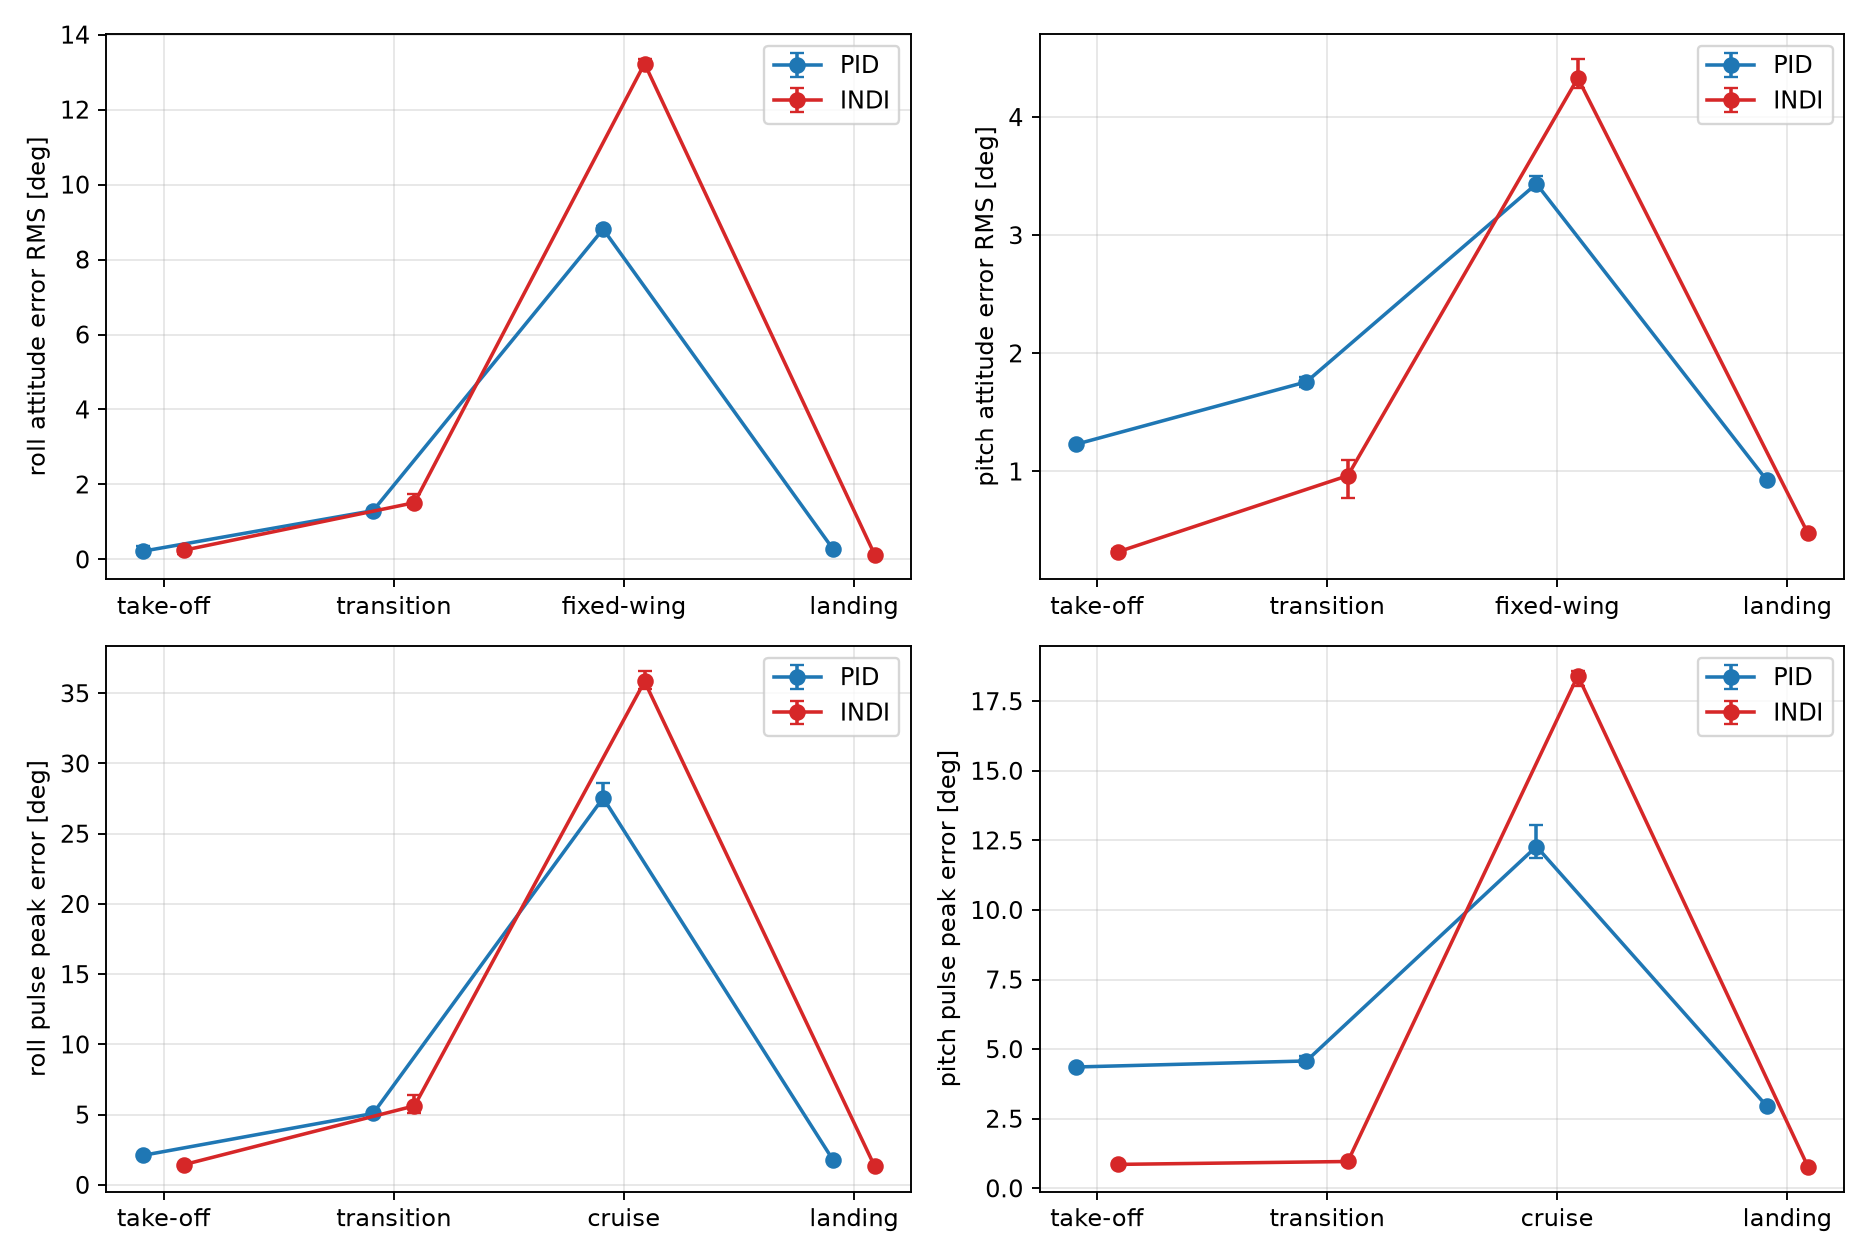
\includegraphics[width=0.95\textwidth]{../runs/noisy_wind/compare/metrics_w6.png}
    \caption{Paired \SI{6}{\meter\per\second} wind experiment: roll and pitch tracking-error RMS by flight phase (upper row), and baseline-subtracted peak error in the five-second window after each scheduled one-second moment pulse (lower row). Points are means of detected pulses, normally over three seeds; whiskers show their minimum and maximum. A few take-off roll markers were not resolved by the lower-rate servo log, so their sample sizes are smaller (one or two; see the per-pulse CSV). Pulse windows are named by their trigger, which can differ from the actual flight phase at injection.}
    \label{fig:crosswind-comparison}
\end{figure}

At \SI{9}{\meter\per\second}, take-off pitch RMS is \SI{2.02}{\degree} for PID and \SI{0.32}{\degree} for INDI; transition roll RMS is \SI{2.71}{\degree} and \SI{1.70}{\degree}. The cruise roll-pulse peak averages \SI{100.67}{\degree} for PID and \SI{25.72}{\degree} for INDI. This is not evidence for an unassisted fixed-wing improvement: the lift motors assisted in the fixed-wing phase for both controllers, averaging \SI{33.4}{\percent} of its duration for PID and \SI{10.6}{\percent} for INDI. Differences in trajectory, transition timing, and assist status limit causal attribution to the rate law alone.

\begin{figure}[H]
    \centering
    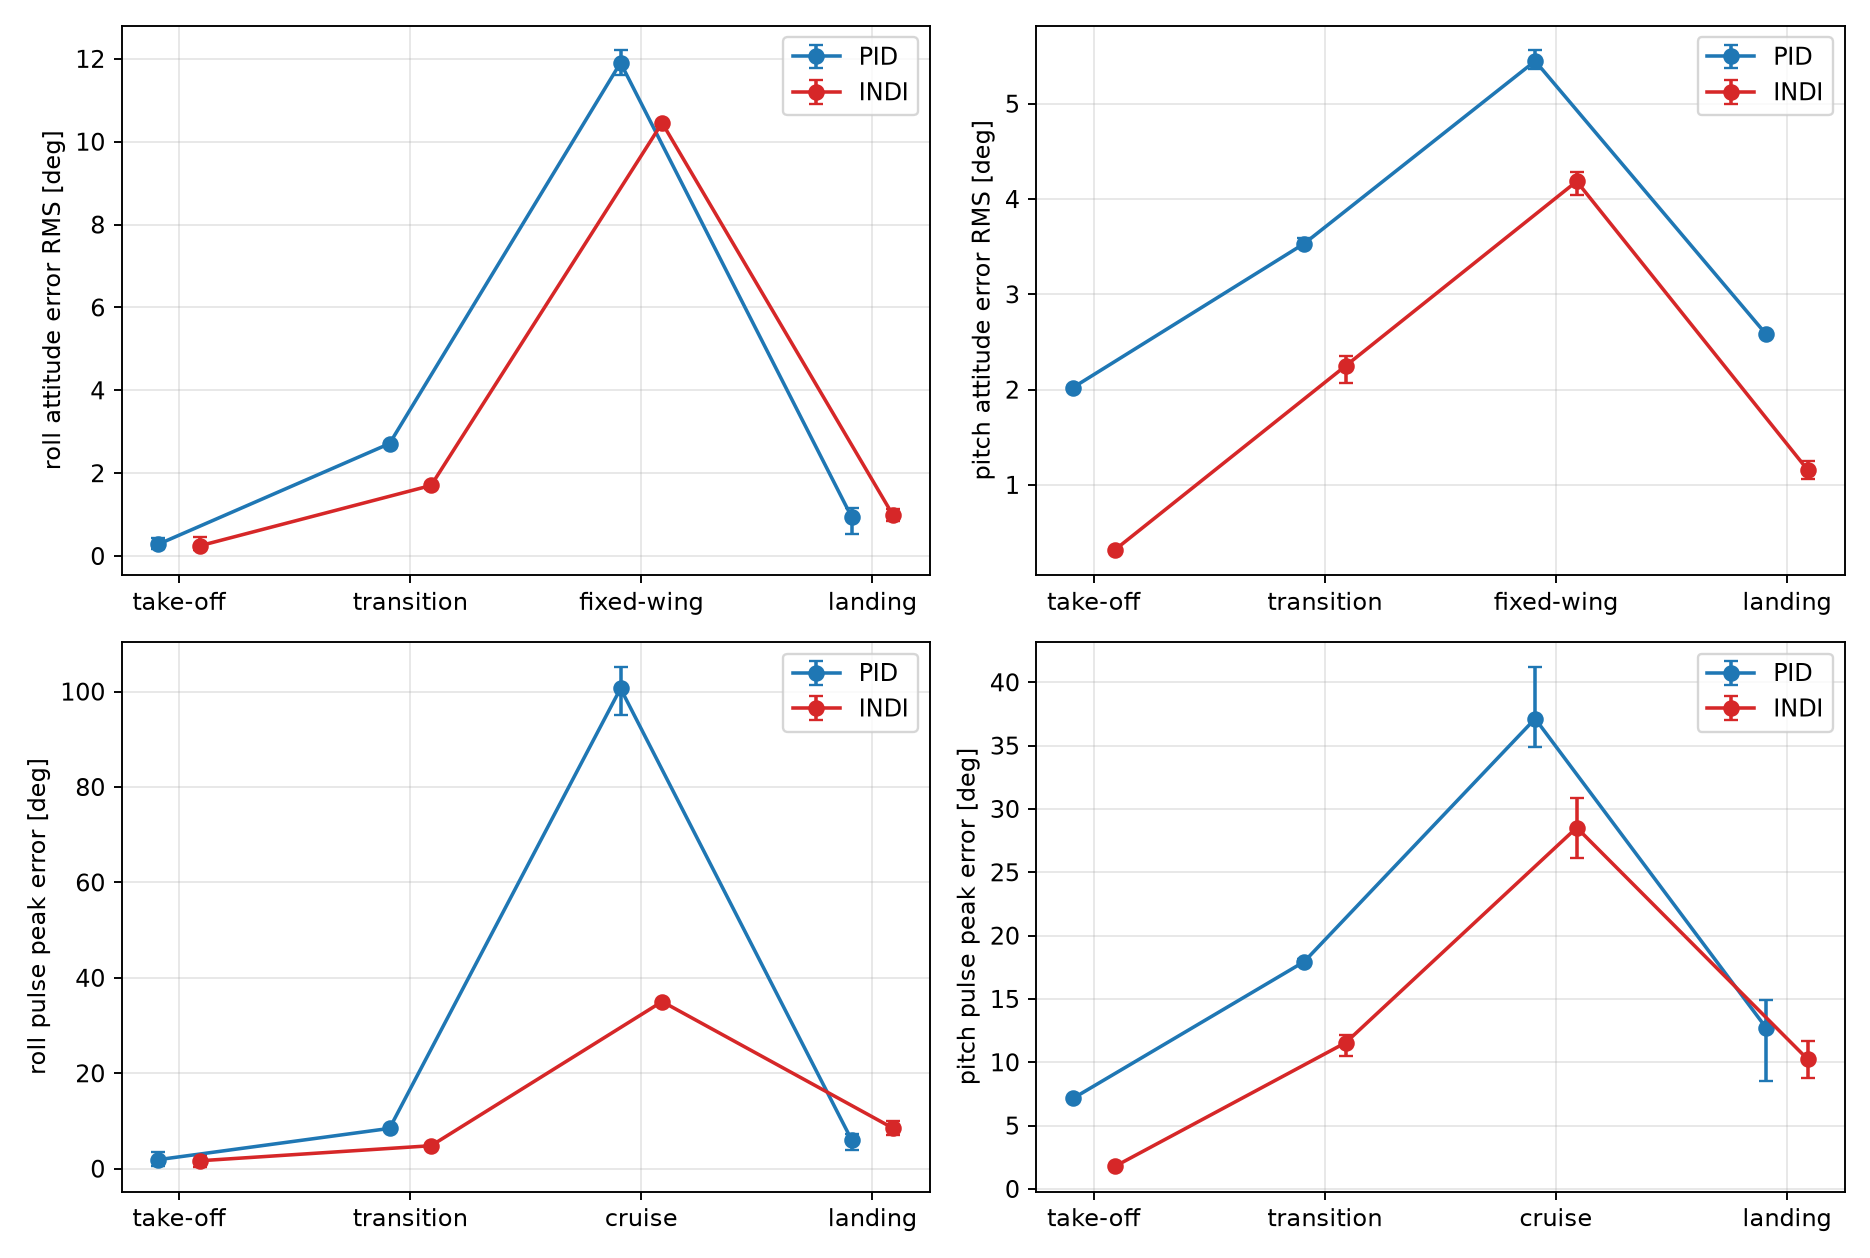
\includegraphics[width=0.95\textwidth]{../runs/noisy_wind/compare/metrics_w9.png}
    \caption{Paired \SI{9}{\meter\per\second} wind experiment with the same definitions as Fig.~\ref{fig:crosswind-comparison}. Three seed-paired, full-physics missions were completed per controller; one take-off roll marker was missed in INDI and the cruise roll-pulse result includes assisted flight, not a purely wing-borne test.}
    \label{fig:crosswind-nine}
\end{figure}

The added Gazebo IMU noise was calibrated separately against a manual airborne hover interval from the real log. In an independent calm validation flight, post-filter \SIrange{20}{120}{\hertz} roll-gyro RMS was \SI{0.251}{\degree\per\second} in simulation versus \SI{0.254}{\degree\per\second} on the aircraft; the pitch gyro remained \SI{0.105}{\degree\per\second} versus \SI{0.060}{\degree\per\second} (\SI{74}{\percent} high). The acceleration-axis RMS values for simulation versus real were $0.177$ versus $0.175$ (x), $0.166$ versus $0.169$ (y), and $0.240$ versus $0.205$ (z), all in \si{\meter\per\second\squared}. The gyro filter, loop rate, harmonic notch and tonal rotor vibrations still differ from the real aircraft; matching integrated noise power is not hardware validation.

\begin{figure}[H]
    \centering
    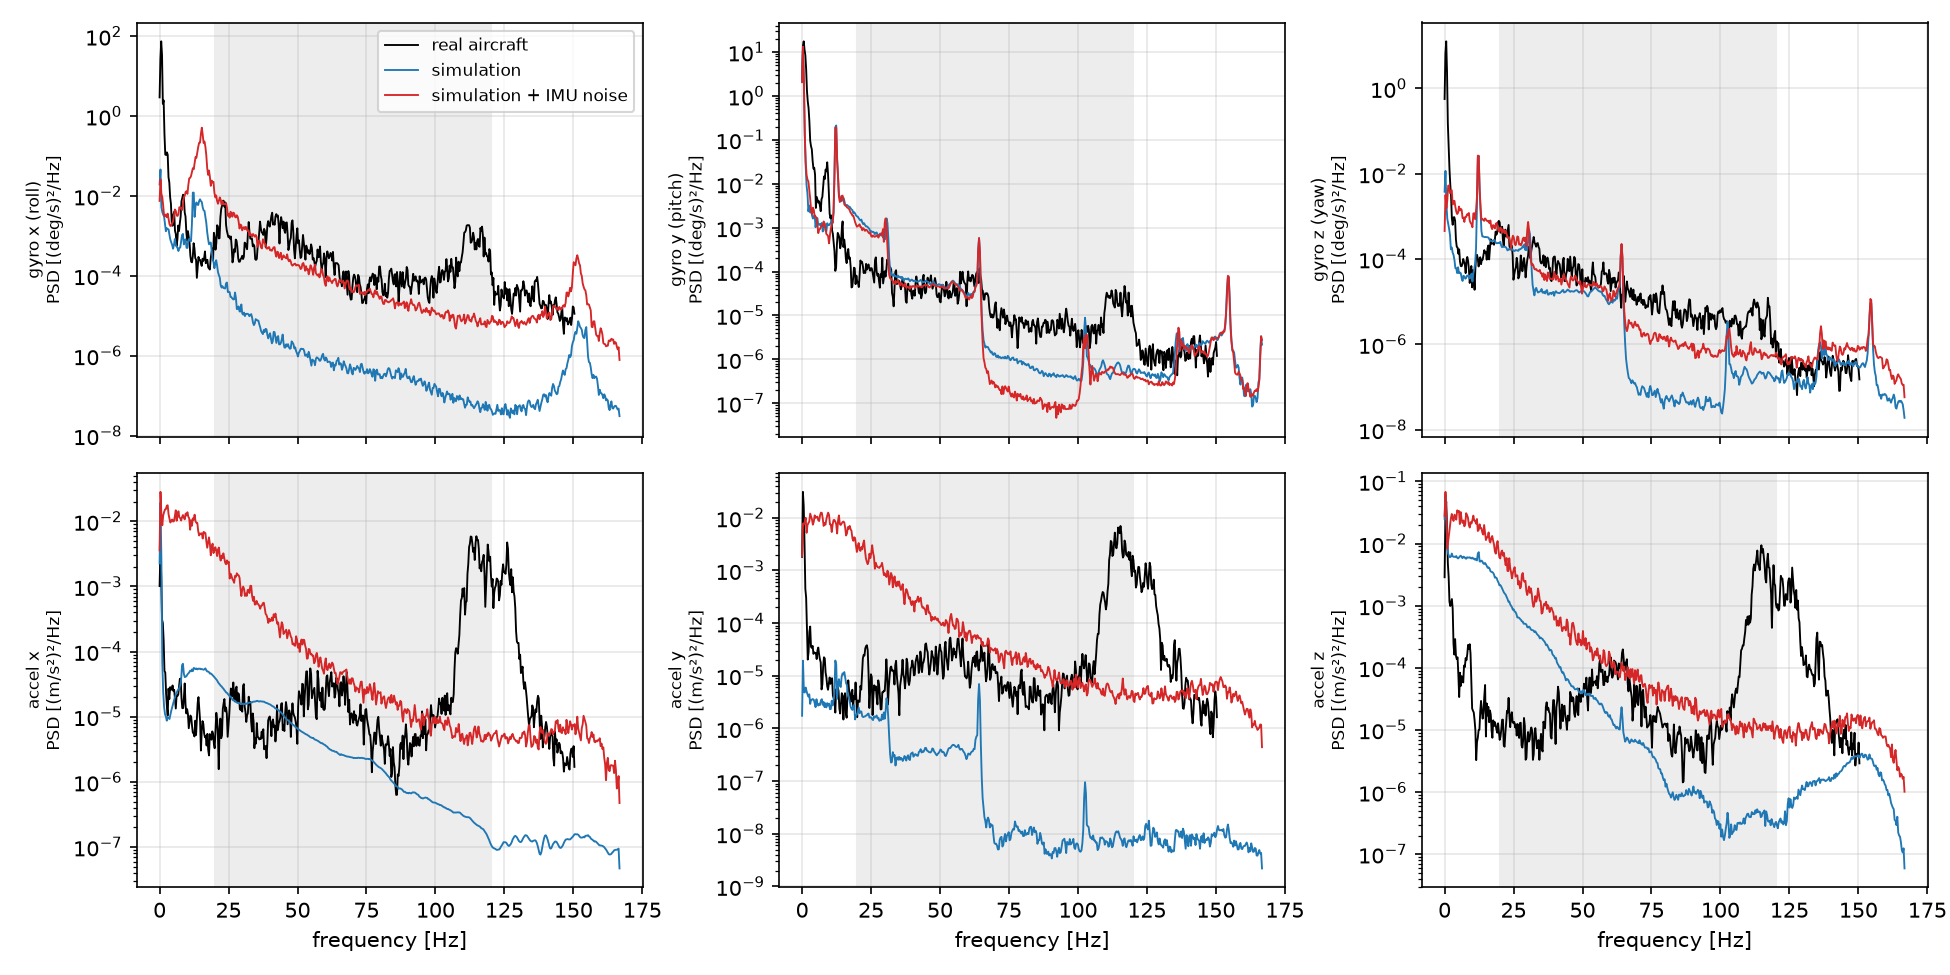
\includegraphics[width=0.98\textwidth]{../runs/noisy_wind/imu_match_final.png}
    \caption{Primary logged IMU spectra in manual real hover, a noise-free simulated square-mission landing hover and an independently flown simulated landing hover with calibrated sensor noise. Shading indicates the \SIrange{20}{120}{\hertz} band integrated for the six-axis RMS comparison. Unlike real motor vibration, the injected sensor noise is Gaussian; spectral shape and pitch-gyro power remain mismatched.}
    \label{fig:noisy-imu-validation}
\end{figure}

\subsection{Discussion of findings}
\label{sec:discussion-findings}
\label{sec:results-smooth-flight}
The real and simulated evidence answer different questions. The physical log is most valuable as a measurement of the hardware environment: it records the gyro-noise floor, filter configuration, scheduler rate, and the fact that the available flight never reached a valid fixed-wing condition. The SITL campaign is most valuable as an integration and handover test: the activity flags show which effector set runs INDI in each phase, and the crab-angle result confirms that the simulated aircraft feels the specified crosswind aerodynamically.

Taken together, the results expose the central sim-to-real risk rather than hiding it. Before noise injection, the original simulator produced roughly 47 times less roll-axis acceleration noise than the physical aircraft in the estimator band. The rerun matches integrated roll-gyro hover noise more closely, but not the real tonal spectrum, pitch-gyro noise, filter chain or airframe plant. The real flight provides no wing-borne data with which to validate the aerodynamic model. The seed-paired moment-pulse results show condition-dependent gains and costs, not a general guarantee of robust control.

The practical conclusion is staged. The present results support further SITL tuning and a better hardware experiment; they do not support a claim of real-flight INDI performance, superior atmospheric gust rejection, or a general PID-versus-INDI advantage. Filter and sensor matching, plant fidelity and a safe real-flight test remain necessary before transferring the controller to the vehicle.

\subsection{Limitations of the study}
\label{sec:limitations}
In the project 
The real dataset contains a manually flown PID record, no measured airspeed, and only \SI{8.4}{\second} in forward flight; it cannot validate the wing, transition, or rate-loop plant. The Gazebo propeller model is valid only over its measured RPM range, and the simulated gyro environment is significantly cleaner than physical model, where noise from the motor and resonance of the frame have a significant role. The Yaw authority problem caused by the twisting of the frame is unmodeled in the simulation. Finally, the weak transition pseudo-control tracking and the failed \SI{9}{\meter\per\second} INDI validation show that the present gains are not a robust final tuning. These limitations bound every performance claim in this thesis.


\subsubsection{Problems encountered during implementation}
\label{sec:filtering-problem}
Beyond the modelling limitations above, several problems were found while getting the controller working. They are reported here because most of them were invisible in the flight itself -- the aircraft completed its mission in every case -- and because the way each was found says something about what a simulation can and cannot be trusted to reveal.

\textbf{The parameter file was never being read.} The SITL defaults file was a five-column QGroundControl export. ArduPilot's parser takes the first whitespace-separated token as the parameter name and the second as its value, so every line asked to set a parameter named after the export's index column. Nothing in the file was applied, and each run instead booted from whatever the previous session had left in the autopilot's stored memory. This is the real explanation for a symptom previously recorded as a single parameter refusing to load from defaults: no parameter was loading, and the ones that appeared correct were leftovers. It also means the configuration of any earlier result is not reconstructible. The file is now two-column, and the run harness gives each case a fresh stored memory so that the defaults file is the only source of parameters.

\textbf{Synchronisation was incomplete, and that was the limit cycle.} The first implementation filtered the acceleration estimate but added the increment to an unfiltered command, which is the defect Section~\ref{sec:synchronization-theory} describes. Correcting it to filter the command with the same estimator filter was necessary but not sufficient: the rate loop still limit-cycled. Two further lags sit between commanding an effector and seeing the moment, and neither was on the command path -- the effector's own response, and the IMU gyro filter. Section~\ref{sec:indi-implementation} gives the analysis; the practical consequence is that with only the estimator filter replayed, the identified plant predicts a phase margin of $-\SI{34}{\degree}$, and the loop oscillated within \SI{10}{\percent} of the predicted frequency. Replaying all three stages removed it.

\textbf{Wind that pushed the aircraft instead of blowing past it.} Gazebo's wind plugin approximates the force on a wind-enabled link as $F = m\,k\,(v_{\mathrm{wind}} - v_{\mathrm{link}})$ with $k=1$ by default, which on the \SI{2.8}{\kilogram} fuselage link is a velocity-proportional drag of roughly \SI{48}{\newton} at cruise against a weight of \SI{31}{\newton}. The forward transition stopped happening entirely. That approximation is intended for objects with no aerodynamic model of their own; this aircraft has a lift-and-drag model on every surface, so the force approximation was disabled and the wind left to act through the air-relative velocity those surfaces already compute (Section~\ref{sec:results-wind}).

\textbf{An oscillation that was not the controller's.} A line near \SI{16}{\hertz} in the hover angular-acceleration estimate was read as an INDI limit cycle through several iterations. Two things eventually contradicted that reading: the frequency did not move when the inversion gain was changed by \SI{35}{\percent}, and the same line is present in the PID baseline when the comparison is made on the raw gyro rather than on the controller's internal estimate -- which only exists while INDI is running, and so had no baseline to be compared against. Measured properly, INDI has \emph{less} energy in that band than the PID. The line is a property of the simulated airframe whose source has not been identified. The lesson is specific and worth stating: a diagnostic computed only inside the controller under test cannot distinguish the controller from the plant.

\textbf{Integration friction.} Several smaller difficulties came from working inside a mature codebase. The INDI controller is built on the attitude controller that ArduPilot already uses for this vehicle class, so only the rate loop is overridden and the angle loop, throttle handling and frame transforms stay stock. The mixer does not store the roll and pitch it actually applied after saturation, so the controller recovers them each cycle from the individual motor outputs. The control loop in SITL does not run at its nominal rate: the simulator steps in whole milliseconds, so a \SI{400}{\hertz} loop actually runs every \SI{3}{\milli\second}. The derivative and every filter corner therefore use the measured loop period, not the nominal one.

\section{Conclusion and Future Work}
\label{sec:conclusion}

This thesis develops an incremental rate-control path for a quadplane, from the control-theory derivation to an INDI rate loop on the lift motors and control surfaces in ArduPilot, handed over between them by ArduPilot's own transition logic. It explains why cascaded PID remains a practical baseline; why a full nonlinear inverse is unsuitable when the aerodynamic model is uncertain; how the incremental law follows from both Taylor-series and sensor-based derivations; and why command, actuator, and measurement delays must be matched for the inversion to remain valid. The controller executes through hover, transition, and forward flight in Gazebo/SITL, with activity logging that separates genuine INDI ownership from PID fallback.

The real flight record constrains, rather than validates, the simulation. It confirms the hardware sensor environment and reveals a filtered roll-axis acceleration-noise level 47 times the calm-SITL value, but it contains neither measured airspeed nor enough fixed-wing operation to validate transition dynamics. Within SITL, the handover engages as designed and the \SI{6}{\meter\per\second} case improves transition attitude RMSE, but the \SI{9}{\meter\per\second} case produces \SI{2.45}{\degree} roll-attitude RMS error and \SI{11.07}{\degree\per\second} roll-rate RMS error. The results therefore demonstrate implementation and expose a robustness limit; they do not demonstrate real-aircraft INDI performance or a general PID-versus-INDI advantage. The immediate next step is a matched, instrumented PID validation flight and its replay in SITL, followed by repeated transient-disturbance experiments only after the model and sensor discrepancy have been addressed.

\subsection{Future work}
\label{sec:future-work}
Most notably, the eventual goal of this line of work is to fly the INDI controller on the real vehicle, not just in simulation. That step is deliberately placed last and is gated on everything above: it should only be attempted once (i) the simulation has been shown to reproduce real PID flight behaviour to an accepted tolerance, especially in yaw (Section~\ref{sec:sim-to-real}), (ii) the corrected synchronization fix of Eq.~\eqref{eq:sync-fix} has been re-validated in SITL, and (iii) the standard hardware-in-the-loop progression is followed: bench and props-off checks, tethered hover, an immediate remote-controlled fallback switch back to PID, and only then a cautious, low-altitude, progressively-expanding real flight-test campaign. Further work beyond the first real flight includes online or scheduled effectiveness identification for the hover and fixed-wing gains alike, especially for yaw, which remains on the stock coordinated-turn law in both regimes (Section~\ref{sec:indi-fw-implementation}); tracking-accuracy validation of the fixed-wing extension against the metrics of Section~\ref{sec:metrics}, beyond the engagement result already obtained (Section~\ref{sec:results-transition}); constrained control allocation for the overactuated transition and cruise mixer; and a genuine outer-loop (vertical/position) INDI law to replace the current bounded PID throttle correction, following the cascaded hover/fixed-wing structure demonstrated for a comparable vehicle by \citet{zhou2023}.

\bibliographystyle{unsrtnat}
\bibliography{thesis}

\appendix
\section{Physical Prototype Build}
\label{sec:appendix-build}
\begin{figure}[H]
    \centering
    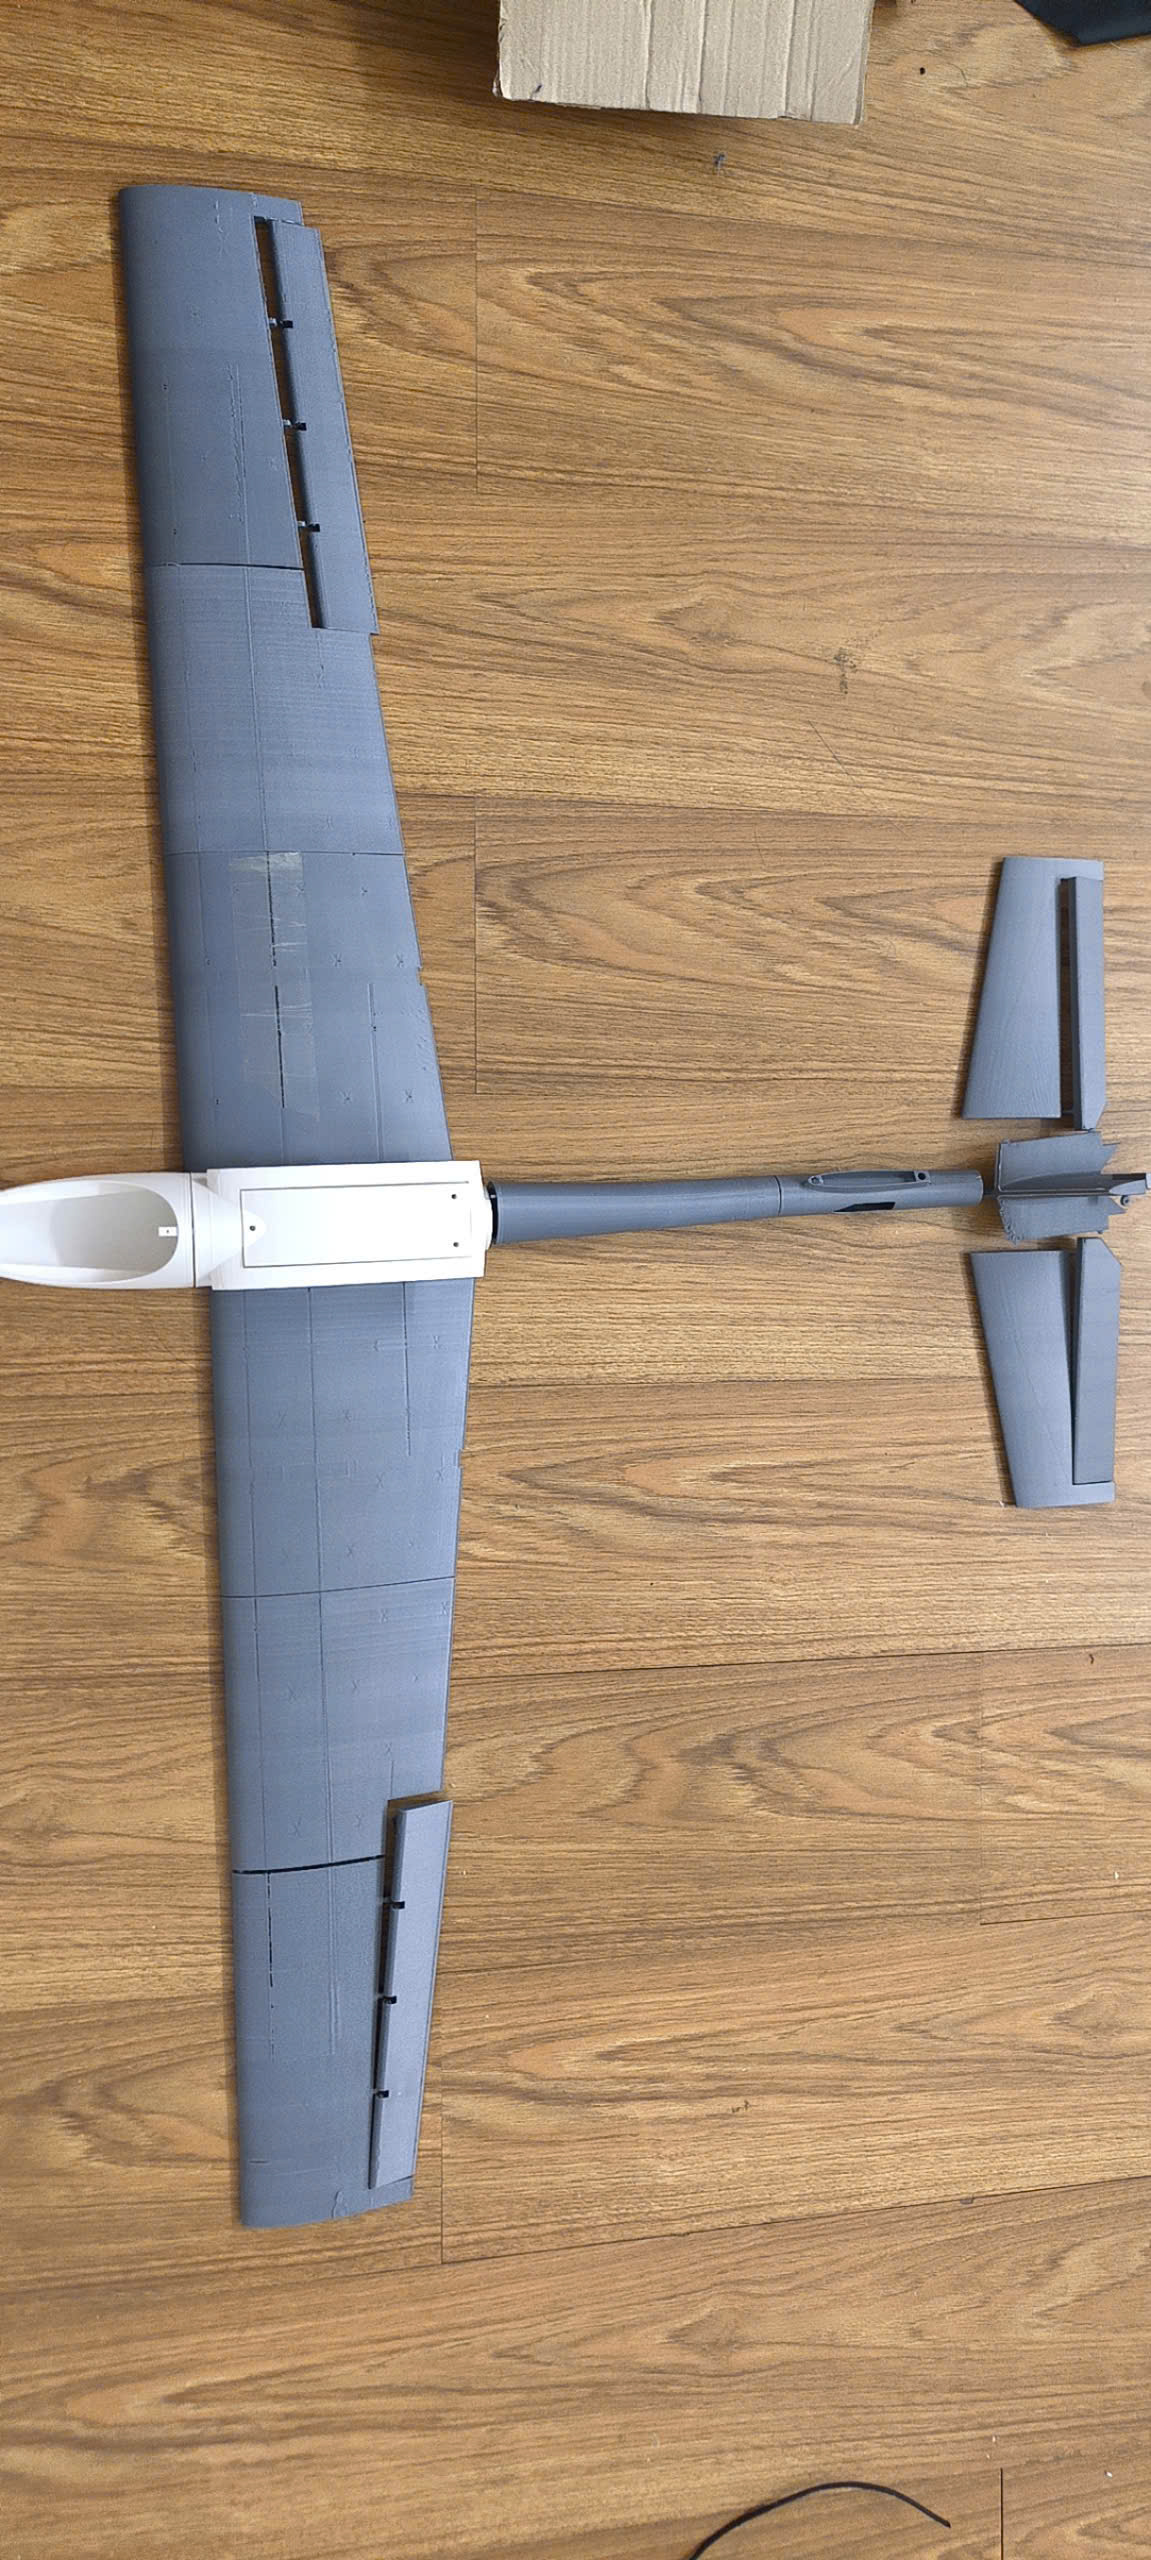
\includegraphics[width=0.85\textwidth]{./images/1st iteration.jpeg}
    \caption{First 3D-printed structural iteration of the wing, boom, and tail assembly, prior to final assembly and avionics integration.}
    \label{fig:first-iteration}
\end{figure}

\section{Vehicle and Controller Parameters}
\label{sec:appendix-parameters}
The PID runs use \texttt{sim/stock\_pid.param}. The INDI runs use the same file with \texttt{sim/indi.param} appended, so the two differ only in the lines of Table~\ref{tab:appendix-indi-params}. With \texttt{Q\_INDI\_ENABLE}\,=\,0 (the default) the INDI code is not loaded and the aircraft runs stock ArduPilot.

\begin{table}[H]
    \centering
    \caption{INDI parameters, as flown (\texttt{sim/indi.param}).}
    \label{tab:appendix-indi-params}
    \begin{tabular}{llll}
        \toprule
        Parameter & Value & Source & Role \\
        \midrule
        \texttt{Q\_INDI\_ENABLE}   & 1 & --- & Load the INDI controller at boot \\
        \texttt{Q\_INDI\_AXES}     & 27 & --- & Bitmask: VTOL roll, VTOL pitch, FW roll, FW pitch \\
        \texttt{Q\_INDI\_FILT\_HZ} & \SI{12.7}{\hertz} & design & Two poles of $H$ (Eq.~\eqref{eq:diagonal-inversion}) \\
        \midrule
        \texttt{Q\_INDI\_RLL\_G}   & 56.7 & identified & Lift-motor roll effectiveness \\
        \texttt{Q\_INDI\_PIT\_G}   & 44.8 & identified & Lift-motor pitch effectiveness \\
        \texttt{Q\_INDI\_YAW\_G}   & 0    & excluded   & Zero keeps yaw on the PID \\
        \texttt{Q\_INDI\_ACT\_TC}  & 0    & identified & Lift-motor lag \\
        \texttt{Q\_INDI\_ACT\_DLY} & \SI{4}{\milli\second} & identified & Lift-motor delay \\
        \texttt{Q\_INDI\_RLL\_K}, \texttt{PIT\_K} & \SI{13.5}{\per\second} & margins & Rate error to $\nu$ \\
        \midrule
        \texttt{Q\_INDI\_FW\_RLL\_G} & 16.7 & identified & Aileron effectiveness at \texttt{SCALING\_SPEED} \\
        \texttt{Q\_INDI\_FW\_PIT\_G} & 12.4 & identified & Elevator effectiveness at \texttt{SCALING\_SPEED} \\
        \texttt{Q\_INDI\_FW\_TC}     & \SI{10}{\milli\second} & identified & Surface servo lag \\
        \texttt{Q\_INDI\_FW\_RLL\_K}, \texttt{FW\_PIT\_K} & \SI{10.5}{\per\second} & margins & Rate error to $\nu$ \\
        \bottomrule
    \end{tabular}
\end{table}

Effectiveness is in \si{\radian\per\second\squared} per unit normalised command: full mixer input for the lift motors, full surface travel for the surfaces. \texttt{SCALING\_SPEED} is \SI{15}{\meter\per\second}; the surface values are divided by the square of ArduPilot's speed scaler, which is Eq.~\eqref{eq:fw-indi-scaling}. ``Identified'' values come from \texttt{analysis/identify\_G.py} on the hover and fixed-wing system-identification runs; ``margins'' are the largest gains with at least \SI{6}{\decibel} gain margin and \ang{45} phase margin from \texttt{analysis/indi\_margins.py}, reduced slightly.
% NOTE 2026-09-26: Section sec:results-identification still quotes G = 61.7 / 55.4 and
% tau = 23 ms from an earlier identification; the flown file uses 56.7 / 44.8, tau 0,
% delay 4 ms. Reconcile the Results text with the identification that produced indi.param.

\begin{table}[H]
    \centering
    \caption{Other settings referred to in the text, as flown (\texttt{sim/stock\_pid.param}).}
    \label{tab:appendix-other-params}
    \begin{tabular}{lll}
        \toprule
        Parameter & Value & Plain name in the text \\
        \midrule
        \texttt{AIRSPEED\_STALL}  & \SI{12}{\meter\per\second} & stall speed \\
        \texttt{AIRSPEED\_MIN}    & \SI{14}{\meter\per\second} & minimum airspeed \\
        \texttt{AIRSPEED\_CRUISE} & \SI{17}{\meter\per\second} & cruise airspeed \\
        \texttt{Q\_ASSIST\_SPEED} & \SI{13}{\meter\per\second} & lift-motor assist speed \\
        \texttt{Q\_OPTIONS}       & 0 (bit 7 cleared) & forced-assist setting (bit 7, \texttt{Q\_ASSIST\_FORCE\_ENABLE}) \\
        \texttt{Q\_TRANSITION\_MS} & \SI{3000}{\milli\second} & timed part of the forward transition \\
        \texttt{SCHED\_LOOP\_RATE} & \SI{400}{\hertz} & nominal control-loop rate \\
        \texttt{INS\_GYRO\_FILTER} & \SI{20}{\hertz} & gyro low-pass filter ($F_g$) \\
        \texttt{WP\_RADIUS}       & \SI{25}{\meter} & waypoint acceptance radius \\
        \texttt{NAVL1\_PERIOD}    & \SI{12}{\second} & navigation look-ahead period \\
        \bottomrule
    \end{tabular}
\end{table}

\section{Names Used in ArduPilot, Gazebo and the Project Files}
\label{sec:appendix-names}
The main text uses plain names. This appendix gives the matching name in the code, the model file or the log. File paths are relative to the \texttt{rework/} folder.

\begin{longtable}{p{0.40\textwidth}p{0.52\textwidth}}
\textbf{Plain name in the text} & \textbf{Name in ArduPilot, Gazebo or the repository} \\
\midrule
\multicolumn{2}{l}{\emph{Flight modes and log messages}} \\
hover mode & \texttt{QHOVER} \\
stabilised fixed-wing mode & \texttt{FBWA} \\
logged airspeed & \texttt{CTUN.As} \\
airspeed-sensor messages & \texttt{ARSP} \\
stored hover throttle & \texttt{Q\_M\_THST\_HOVER} \\
batch-sampled gyro log & \texttt{INS\_LOG\_BAT\_MASK} \\
logged vibration levels & \texttt{VIBE.VibeX/Y/Z} \\
logged body rates & \texttt{RATE} \\
parameters written at boot & \texttt{PARM} \\
INDI log, lift motors / surfaces & \texttt{INDI} / \texttt{INDF} \\
\midrule
\multicolumn{2}{l}{\emph{Controller code (branch \texttt{indi})}} \\
INDI core, one per axis & \texttt{AC\_INDI\_Axis} (\texttt{AC\_INDI.cpp}) \\
INDI parameter block & \texttt{AC\_INDI\_Params}, parameters \texttt{Q\_INDI\_*} \\
lift-motor INDI rate loop & \texttt{AC\_AttitudeControl\_INDI::rate\_controller\_run\_dt()}, derived from \texttt{AC\_AttitudeControl\_TS} \\
surface INDI rate loop & \texttt{AP\_FW\_Controller::run\_rate\_control()} \\
boot-time switch & \texttt{QuadPlane::setup()} reading \texttt{Q\_INDI\_ENABLE} \\
applied mixer input $u_{\mathrm{applied}}$ & \texttt{AC\_AttitudeControl\_INDI::applied\_input()} \\
\midrule
\multicolumn{2}{l}{\emph{Gazebo model (\texttt{sim/gazebo\_models/VTOL\_Quadplane/model.sdf})}} \\
lift-drag system & \texttt{gz-sim-lift-drag-system} \\
$S$, $\alpha_0$, $C_{L\alpha}$, $C_{D\alpha}$, $C_{m\alpha}$ & \texttt{area}, \texttt{a0}, \texttt{cla}, \texttt{cda}, \texttt{cma} \\
$\alpha_{\mathrm{stall}}$, post-stall slopes & \texttt{alpha\_stall}, \texttt{cla\_stall}, \texttt{cda\_stall}, \texttt{cma\_stall} \\
$\mathbf{r}_{cp}$, $\hat{\mathbf{e}}_f$, $\hat{\mathbf{e}}_u$ & \texttt{cp}, \texttt{forward}, \texttt{upward} \\
$k_\delta$ & \texttt{control\_joint\_rad\_to\_cl} \\
servo scaling & \texttt{ArduPilotPlugin} \texttt{<multiplier>}, \texttt{<offset>} \\
Gazebo wind plugin & \texttt{WindEffects}, links with \texttt{enable\_wind} \\
\midrule
\multicolumn{2}{l}{\emph{Files and scripts}} \\
square mission & \texttt{sim/square.plan} \\
zigzag mission & \texttt{sim/Default square zigzag path.plan} \\
mission runner, pulse schedule & \texttt{sim/fly\_plan\_mission.py} (class \texttt{Disturbance}) \\
torque injection & \texttt{sim/disturb.py} \\
lifting-surface ranking & \texttt{analysis/auxiliary/rank\_lifting\_surfaces.py} \\
mission geometry & \texttt{analysis/auxiliary/plan\_geometry.py} \\
autopilot stored memory & \texttt{eeprom.bin} \\
\end{longtable}

\section{Transition Control Hooks}
\label{sec:appendix-transition-hooks}
The effector-ownership rule of Listing~\ref{lst:ownership} is evaluated in \texttt{Plane::stabilize()} (\texttt{ArduPlane/Attitude.cpp}) every loop:

\begin{lstlisting}[style=pseudostyle, caption={Surface INDI permission, as in \texttt{Plane::stabilize()}.}, label={lst:fw-indi-gate}]
fw_indi = quadplane.available() and Q_INDI_ENABLE > 0
          and not quadplane.in_vtol_mode()
          and quadplane.transition->complete()
          and not quadplane.in_assisted_flight()
rollController.set_indi(params, ROLL,  fw_indi and FW_ROLL  in Q_INDI_AXES)
pitchController.set_indi(params, PITCH, fw_indi and FW_PITCH in Q_INDI_AXES)
\end{lstlisting}

\begin{longtable}{p{0.34\textwidth}p{0.58\textwidth}}
\textbf{Name} & \textbf{Function} \\
\midrule
\texttt{in\_vtol\_mode()} & True in any hover flight mode (take-off, landing, hover). \\
\texttt{transition->complete()} & True once the forward transition has finished. \\
\texttt{in\_assisted\_flight()} & True while the lift motors help the wing (below \texttt{Q\_ASSIST\_SPEED}, or forced by \texttt{Q\_OPTIONS} bit 7). \\
\texttt{SLT\_Transition} & Transition state machine: wait for airspeed, timed handover (\texttt{Q\_TRANSITION\_MS}), done. \\
\texttt{AIRSPEED\_MIN} & Airspeed at which the airspeed wait ends. \\
\texttt{set\_indi()} & Tells a surface rate controller whether INDI may run this cycle; otherwise the stock PID runs. \\
\end{longtable}

The lift-motor loop needs no gate of its own: when the transition is complete and assist is off, ArduPilot stops running the VTOL rate loop, and \texttt{AC\_AttitudeControl\_INDI} additionally falls back to the PID whenever the motors are not fully spun up.

\section{Gazebo, SITL, and MAVLink Configuration}
\label{sec:appendix-config}
This appendix will reproduce the relevant SDF blocks (lift-drag plugin parameters per surface, motor/propeller plugin parameters, sensor rates), the ArduPilot parameter file, the MAVLink/serial port configuration used to connect SITL to Gazebo, and the exact launch commands, once the corresponding files are finalised.

\section{Additional Derivations and Pseudocode}
\label{sec:appendix-derivations}
Listing~\ref{lst:indi-pseudocode} gives the per-cycle update of one INDI axis (\texttt{AC\_INDI\_Axis::update()}), including the command synchronisation of Eq.~\eqref{eq:sync-fix}, and the per-axis fallback of the lift-motor loop.

\begin{lstlisting}[style=pseudostyle, caption={One INDI axis, one call per control cycle.}, label={lst:indi-pseudocode}]
function indi_axis_update(rate, u_applied, nu, G, dt):
    # dt is the measured loop period (3 ms in SITL, not the nominal 2.5 ms)
    u_act   = actuator_model(u_applied)         # A: delay, then first-order lag
    u_gyro  = gyro_filter_copy(u_act)           # F_g: same low-pass as the gyro
    u0_f    = H(u_gyro)                         # H: two poles at FILT_HZ
    wdot    = (rate - rate_prev) / dt           # backward difference
    wdot_f  = H(wdot)                           # same H as the command path
    rate_prev = rate
    return u0_f + (nu - wdot_f) / G             # new normalised command

function lift_motor_rate_loop(rate_target, gyro, dt):       # every VTOL cycle
    for axis in (roll, pitch, yaw):
        u_applied = recovered_from_motor_outputs(axis)
        if motors_spooled and axis in Q_INDI_AXES and G[axis] > 0:
            nu = K[axis] * (rate_target[axis] - gyro[axis])
            out[axis] = indi_axis_update(gyro[axis], u_applied, nu, G[axis], dt)
            pid[axis].reset_integrator()         # bumpless hand-back
        else:
            out[axis] = pid[axis].update(rate_target[axis], gyro[axis])
            indi[axis].reset(gyro[axis], u_applied)   # bumpless switch-in
    mixer.set(out)

function surface_rate_loop(axis, rate_target, rate, speed_scaler, dt):
    if fw_indi_allowed(axis) and speed_scaler > 0 and FW_G[axis] > 0:
        G  = FW_G[axis] / speed_scaler^2          # Eq. (fw-indi-scaling)
        nu = FW_K[axis] * (rate_target - rate)
        return indi_axis_update(rate, u_last, nu, G, dt)
    return stock_pid(axis)                         # INDI states follow the PID
\end{lstlisting}

\end{document}
